\documentclass[11pt]{amsart}
\usepackage{amssymb,bm}%,enumitem}
\usepackage{amsmath}
\usepackage{amsfonts}
\usepackage{amsthm}
\usepackage{color}
\usepackage{graphics,graphicx,url}
\usepackage{enumerate}
\usepackage{comment}
\usepackage{subcaption}
\usepackage{thmtools}
\usepackage{thm-restate}

\usepackage{centernot}


\usepackage{breqn} %% Break long equations, use dmath



\usepackage{xcolor}
\newcommand{\jen}[1]{{\textcolor{blue}{#1}}}
\newcommand{\mee}[1]{\textcolor{magenta}{{#1}}}
\newcommand{\dbb}[1]{\textcolor{cyan}{{#1}}}





\usepackage{tikz}
\usetikzlibrary{calc,decorations.pathmorphing,patterns,arrows,decorations.markings,positioning}
\usetikzlibrary{automata,chains,fit,shapes}


\renewcommand{\subjclassname}{%
  \textup{2020} Mathematics Subject Classification}

\usepackage{graphicx,pdflscape,rotating,float}
\usepackage{enumitem}
\pagestyle{plain}




% definitions
\newcommand{\bi}{\begin{itemize}}
\newcommand{\ei}{\end{itemize}}
\newcommand{\be}{\begin{enumerate}}
\newcommand{\ee}{\end{enumerate}}
\newcommand{\bc}{\begin{center}}
\newcommand{\ec}{\end{center}}
\newcommand{\bt}{\begin{tabular}}
\newcommand{\et}{\end{tabular}}
\newcommand{\ba}{\begin{array}}
\newcommand{\ea}{\end{array}}


\newcommand{\Cpsi}{m}%{C_{S,\psi}}
\newcommand{\Dpsi}{e}%{D_{S,\psi}}
\newcommand{\cA}{c}
\newcommand{\cB}{d}
\newcommand{\cC}{\varsigma}
\newcommand{\nD}{n_0}
\newcommand{\preceqD}{\preceq_2}
\newcommand{\approxD}{\approx_2}
\newcommand{\preceqF}{\preceq_1}
\newcommand{\npreceqF}{\npreceq_1}
\newcommand{\approxF}{\approx_1}
\newcommand{\succeqF}{\succeq_1}
\newcommand\BaumGroup{{\mathfrak G}_{G,H,S}}
\newcommand\Olshan{Ol'shanskii}


\newenvironment{proof*}[1]
  {\renewcommand{\proofname}{#1}%
   \begin{proof}}
  {\end{proof}}



\newtheorem{theorem}{Theorem}[section]
\newtheorem{theoremx}{\bfseries Theorem}
\newtheorem{lemma}[theorem]{Lemma}
\newtheorem{conjecture}[theorem]{Conjecture}
\newtheorem{question}[theorem]{Question}
\newtheorem{proposition}[theorem]{Proposition}
\newtheorem{corollary}[theorem]{Corollary}
\theoremstyle{definition}
\newtheorem{remark}[theorem]{Remark}
\newtheorem{definition}[theorem]{Definition}
\newtheorem{example}[theorem]{Example}


\renewcommand{\thetheoremx}{\Alph{theoremx}} % "letter-numbered" theorems




\usepackage[normalem]{ulem}





\DeclareMathOperator{\aff}{Aff}
\newcommand\f{\varphi}
\newcommand\Z{\mathbb Z}
\newcommand\N{\mathbb N}
\newcommand\Q{\mathbb Q}
\newcommand\R{\mathbb R}
\newcommand\Rplus{\mathbb R^+}
\newcommand\C{\mathbb C}
\newcommand\shuffle{\otimes}
\newcommand\dom{\mathrm{dom}}
\newcommand\pn{\prec_\nsim}
\newcommand\support{\mathrm{supp}}


\newcommand\h{x}



\newcommand\Sph{\text{Sph}}
\newcommand\GA{graph-automatic}
\newcommand\distfun{Cayley distance function}
\newcommand\Distfun{Cayley distance function}
\newcommand\strongGA{strong graph-automatic}
\newcommand\B{\mathcal B}
\newcommand\F{\mathcal F}
\newcommand\E{\mathcal E}\newcommand\D{\mathcal D}

\newcommand\BT{Berdinsky and Trakuldit}

\newcommand{\ii}{\mathfrak{i}}
\newcommand{\cc}{\mathfrak{c}}
\newcommand\hh{h_{G \wr H}}

\renewcommand{\geq}{\geqslant} \renewcommand{\leq}{\leqslant} \renewcommand{\ge}{\geqslant} \renewcommand{\le}{\leqslant}





\title{Separating automatic from \\ Cayley automatic groups}

\author[D. Berdinsky]{Dmitry Berdinsky\textsuperscript{a,b}}
\address{\textsuperscript{a}Department of Mathematics,
		Faculty of Science,
		Mahidol
		University, Bangkok, 10400, Thailand
		\textsuperscript{b}Centre of Excellence in Mathematics,
		Commission on Higher Education, Bangkok, 10400, Thailand}
\email{berdinsky@gmail.com}

\author[M. Elder]{Murray Elder}\thanks{The second author is supported by Australian Research Council grant DP160100486}
\address{School of Mathematical and Physical Sciences, University of Technology Sydney, Ultimo, NSW 2007, Australia}
\email{murray.elder@uts.edu.au}



\author[J. Taback]{Jennifer Taback}\thanks{The third author acknowledges support from Simons Foundation
grant 31736 to Bowdoin College.}
\address{Department of Mathematics,
Bowdoin College, 8600 College Station, Brunswick, ME 04011, USA} \email{jtaback@bowdoin.edu}

\date{\today}

\subjclass[2020]{20E22, 20F10, 20F65, 68Q45}

\keywords{Automatic group; Cayley automatic group; Cayley distance function; Dehn function; wreath product}

\begin{document}

\begin{abstract}
We investigate the problem of distinguishing non-automatic Cayley automatic groups from automatic groups.
It is well known that automatic groups are finitely presented with either linear or quadratic Dehn function.
In this work we show that any Cayley automatic group with Dehn function that is not {\em almost quadratic}, or is not finitely presented, is quantitatively separated from the class of automatic groups via a {\em distance function} previously introduced by the first author and Trakuldit.

For each such group
we construct a concrete unbounded function, depending only on the group,
so that the distance function for any Cayley automatic structure on the group is bounded below by this function.






\end{abstract}

\maketitle




\section{Introduction}
\label{sec:intro}



Cayley automatic groups, introduced by Kharlampovich, Khoussainov
and Miasnikov in \cite{KKMjournal}, generalize the class of automatic groups while retaining some key algorithmic properties.  Namely, the
word problem in a Cayley automatic group is decidable in quadratic time, and the first order theory for a (directed, labeled) Cayley graph of a Cayley automatic group is decidable. The family of Cayley automatic groups is much broader than that of automatic groups, for example it  includes all finitely generated nilpotent
groups of nilpotency class
two \cite{KKMjournal}, the Baumslag-Solitar groups \cite{BerK-BS,KKMjournal},
higher rank lamplighter groups \cite{Taback18}, and wreath products of the form $G\wr \Z$ where $G$ is Cayley automatic  \cite{berdkhouss15}.


An automatic group $G$ is a
group with a regular normal form over a finite generating set $S$, with, for each generator $x\in S$, a finite state automaton  recognizing pairs of normal form words which differ by multiplication by $x$.
In a Cayley automatic group, we allow the normal form to be created from an alphabet of symbols which are {\em a priori} not elements of the group, and define a bijective
function $\psi$ which maps a symbol word to the group element it represents.
Following \cite{measuringcloseness} we assign group elements to the symbol alphabet and enlarge the generating set  to a set $S$ which includes these symbols.
It is then possible to measure the distance in the Cayley graph
with respect to $S$
 between the terminal vertex of the ``symbol word" representing the element and the vertex corresponding to the element itself.
Following \cite{measuringcloseness} we define a function $h_{S,\psi}(n)$ which computes the maximum distance between a group element and its corresponding symbol word, over all symbol words of length at most $n$.
This function is dependent on the generating set $S$ as well as the Cayley automatic structure.
We call $h_{S,\psi}$ the {\em \distfun} associated to the Cayley automatic structure.
Our goal is to use this function to quantitatively separate Cayley automatic groups from automatic groups.

The first author and  Trakuldit proved in \cite{measuringcloseness} that if $G$ has a Cayley automatic structure for which the \distfun\ $h_{S,\psi}$  is bounded above by a constant function, then $G$ is automatic.
It follows that if $G$ is not automatic, then for each Cayley automatic structure on $G$ the corresponding \distfun\ $h_{S,\psi}$ is unbounded.
However, it may be the case that $G$ is  not automatic and admits an infinite sequence of Cayley automatic structures with \distfun s $h_{S_i,\psi_i}$ which get arbitrarily close to a constant function as $i$ approaches infinity.



In this paper we prove that this limiting situation cannot occur for groups which have  super-quadratic Dehn function (see Definition~\ref{defn:strong-super}).
More precisely, we have the following.



We say a Cayley automatic
group $G$ is {\em $f$-separated}
(Definition~\ref{defn:isep}) if the \distfun\ with respect to any Cayley automatic structure on $G$ is bounded below by a function in the equivalence class $[f]$, where the equivalence relation is given in Definition~\ref{defn:equivF} below.
Let $\ii$ denote the function $\ii(n)=n$ on some domain $[N,\infty)$.
Strongly-super-polynomial functions, referred to in Theorem~\ref{thmA:fp} below, are introduced in Definition~\ref{defn:strong-super}.




\begin{restatable}[Separation for finitely presented groups]{theoremx}{ThmA}
\label{thmA:fp}
If $G$ is a finitely presented Cayley automatic group with super-quadratic Dehn function,
 then there exists an unbounded function $\phi$ depending only on $G$ so that $G$ is $\phi$-separated.
 Furthermore, if $G$ has strongly-super-polynomial Dehn function, then  $G$ is $\ii$-separated.
\end{restatable}



 The analogous theorem for non-finitely presented groups is as follows.
A non-finitely presented group is {\em dense} if its irreducible relators have lengths which are ``dense" in the natural numbers; see \S\!~\ref{sec:dense} for a  precise definition.  Wreath products are the prototypical examples of dense groups.



\begin{restatable}[Separation for non-finitely presented groups]{theoremx}{ThmB}
\label{thmB:nfp}
If $G$ is a Cayley automatic group which is not finitely presented, then there is a non-decreasing step function $\phi$ depending only on $G$
that is  linear for infinitely many values,
so that $G$ is $\phi$-separated.
Furthermore, if $G$ is dense then $G$ is $\ii$-separated.
\end{restatable}




We conjecture the following.
\begin{conjecture}\label{conj:1}
Let $G$ be a  Cayley automatic group. Then either $G$ is automatic or $G$ is $\ii$-separated.
\end{conjecture}

Our results provide  support for this conjecture by exhibiting lower bounds for \distfun s  for all non-automatic Cayley automatic groups whose Dehn function is super-quadratic or are not finitely presented.  However, these bounds are not always equivalent to $\ii$.

Groups with quadratic
Dehn function which are not known to be automatic are enticing objects of study as we consider this conjecture.
To date we know of only two classes of such examples that admit a Cayley automatic structure:
\bi[itemsep=5pt]
\item the higher Heisenberg groups  $H_{2k+1}$ for $k\geq 2$ \cite{MR1616147,MR1253544,MR1698761}. These are nilpotent of step 2  so they are Cayley automatic by  \cite[Theorem 12.4]{KKMjournal}. Since the only nilpotent automatic groups are virtually abelian \cite{Epsteinbook}, they are not automatic.

\item the higher rank lamplighter groups, or {\em Diestel-Leader groups}, proven by B\'{e}rub\'{e}, Palnitkar and   the third author in \cite{Taback18}. One can show that the Cayley automatic structure constructed in  \cite{Taback18} has Cayley distance function equivalent to the identity function. These groups are not of type FP$_\infty$ \cite{BartholdiNW}, hence not automatic.
\ei



Further examples of non-automatic groups with quadratic Dehn function include Stallings' group and its generalizations \cite{CarterForester,DisonElderRileyYoung}. These examples are not of type FP$_\infty$, hence not automatic. It is not known whether
these groups admit Cayley automatic structures.


Thompson's group $F$ has quadratic Dehn function and is not known to be automatic or Cayley automatic; it is shown to be 1-counter-graph automatic in \cite{cga}.

\Olshan\ and Sapir \cite{OSapir-CP} give an example of a group with quadratic Dehn function and unsolvable conjugacy problem.
\Olshan\ in \cite{WeirdQuadDehn,Ol-almost} also gives an example which is {\em almost quadratic}
to which  Theorem~\ref{thmA:fp} does not apply; see \S\!~\ref{sec:FP} below.  It is not known whether these groups are automatic or Cayley automatic.
Note that it is equivalent to say that a group is super-quadratic in our definition below and not almost quadratic, as shown in Lemma~\ref{lem:equiv-super-quad}.

We summarize the above discussion in the following question.
\begin{question}\label{qn:1}
Is there a Cayley automatic group with quadratic (or almost quadratic) Dehn function that is not automatic?
\end{question}

In the final section of this paper we prove a result which generalizes a result of the first author and
Khoussainov \cite{berdkhouss15} and adds to the list of known Cayley automatic groups.




\begin{restatable}[Wreath products with virtually infinite cyclic groups]{theoremx}{ThmC}
\label{thmC:wreath}
Let $G$ be a Cayley automatic group, and $H$ any virtually infinite cyclic group.  Then $G \wr H$ is Cayley automatic and $\ii$-separated.
\end{restatable}





\section{Automatic and Cayley automatic groups}
\label{sec:Auto-CGA}


We assume that the reader is familiar with the notions of regular languages, finite automata and  multi-tape synchronous automata.  For more details, we refer the reader to \cite{Epsteinbook}. We say a language $L\subseteq X^n$ is regular if it is accepted by a synchronous $n$-tape automaton where $n\in\N$ and $X$ is a finite set, or {\em alphabet}.

For any group $G$ with finite symmetric generating set $S=S^{-1}$, let $\pi\colon S^*\to G$ denote the canonical projection map. For $w\in S^*$ let $|w|_S$ denote the length of $w$ as a word in the free monoid $S^*$, that is, $|w|_S$ denotes the number of letters in the word $w$.


\subsection{Automatic and Cayley automatic groups}

We define automatic and Cayley automatic groups, and provide some standard lemmas on the invariance of the  Cayley automatic structure under change of generating set.

\begin{definition}
\label{def:aut}
An {\em automatic structure} for a group $G$ is a pair $(S,L)$ where
\be
\item $S$ is a finite symmetric generating set for $G$;
\item $L\subseteq S^*$ is a regular language;
\item  $\pi|_L \colon L \rightarrow G$ is
a bijection;
\item for each $a \in S$ the binary relation
$$R_a = \{(u,v) \in L \times L \mid \pi(u)a=_G\pi(v)\} \subseteq S^* \times S^*$$
is regular, that is, recognized by a two-tape synchronous automaton.
\ee
A group is called {\em automatic} if it has an automatic structure with respect to some finite generating set.
\end{definition} It is a standard result, see, for example \cite[Theorem 2.4.1]{Epsteinbook}, that if $G$ is automatic  then $G$ has an automatic structure with respect to any finite generating set.


Cayley automatic groups were introduced in \cite{KKMjournal} with the motivation of
allowing the language $L$ of normal forms representing group elements to be defined over a
symbol alphabet $\Lambda$ rather than a generating set $S$ for $G$.


\begin{definition}
\label{def:Caut}
A {\em Cayley automatic structure} for a group  $G$ is a 4-tuple  $(S,\Lambda, L,\psi)$ where
\be
\item $S$ is a finite symmetric generating set for $G$;
\item  $\Lambda$ is an alphabet and
 $L \subseteq \Lambda^*$  is a regular
language;
\item
$\psi\colon L \rightarrow G$ is a bijection;
\item
for each $a \in S$
the binary relation
$$R_a = \{(u,v) \in L \times L \,
|\,\psi(u)a=_G\psi(v)\} \subseteq \Lambda^* \times \Lambda^*$$
is regular, that is, recognized by
a two-tape synchronous automaton. \ee

A group is called {\em Cayley automatic} if it has a Cayley automatic structure   $(S,\Lambda, L,\psi)$  with respect to some finite generating set $S$.\end{definition}
As for automatic groups, if $G$ has a  Cayley automatic structure    $(S,\Lambda, L,\psi)$
and $Y$ is another finite generating set for $G$, then there exists a Cayley automatic structure    $(Y,\Lambda_Y, L_Y,\psi_Y)$ for $G$. See \cite[Theorem 6.9]{KKMjournal} for a proof of this fact; we sharpen this in Proposition~\ref{prop:modifyingCAstructure} below.


Note that a Cayley automatic structure $(S,S,L,\pi|_L)$ for $G$, that is, one in which the symbol alphabet is in fact a generating set, and the natural projection gives a bijection from $L$ to $G$, is simply an automatic structure for $G$.

{\em A priori} the symbol alphabet $\Lambda$ has no relation to a generating set for $G$.
However it is straightforward to show that we may assume without loss of generality that $\Lambda=S$ in any Cayley automatic structure.  This is proven in \cite{measuringcloseness} and in Proposition~\ref{prop:modifyingCAstructure} below.
With this assumption, a word $w\in L$ labels a path from $1_G$ to $\pi(w)$ in the Cayley graph $\Gamma(G,S)$.
It is crucial to note that in general $\pi(w)\neq \psi(w)$.



\begin{definition}
\label{def:h}
Let $(G,S)$ be a group with Cayley automatic structure $(S,S, L,\psi)$.  The {\em \distfun}  corresponding to $\psi$ is defined to be
$$ h_{S,\psi}(n) = \max \{ d_S (\pi (w),\psi(w)) \,| \, w \in L^{\leqslant n}\}$$
where $d_S$ is the word  metric on $G$ with respect to $S$ and
$$L^{\leqslant n} = \{ w \in L \, |\, |w|\leqslant n\}.$$
\end{definition}
Let $ \F$ be the following set of non–decreasing functions.
\[ \F=\{f :[N,+\infty)\to \Rplus \mid [N,+\infty)\subseteq \N\wedge \forall n (n\in \mathrm{dom} f \Rightarrow f(n)\leq f(n+1))\}.\]
As noted previously, let $ \mathfrak{i}\in  \F$ denote the identity function $ \mathfrak{i}(n)=n$ on any suitable domain.
Note that if
$G$ is a group with Cayley automatic structure $(S,S,L,\psi)$ and \distfun\ $h_{S,\psi}$, then  $h_{S,\psi}\in \F$.


We introduce the following partial order on $\F$.


\begin{definition}\label{defn:equivF} Let $f,g \in   \F$. We say that $g \preceqF f$ if there exist positive integers $K,M$ and $N$ such that $[N,+\infty) \subseteq
\mathrm{dom}\,g\cap \mathrm{dom}\, f$ and $g(n)\leq Kf(Mn)$ for every integer $n\geq N$.
We say that $g \approxF f$ if $g \preceqF f$ and $f \preceqF g$.
\end{definition}
The subscript in Definition~\ref{defn:equivF} serves to distinguish this equivalence from the equivalence on Dehn functions discussed in \S\!~\ref{subsec:Dehn}.  It is clear from the definition that $\approxF$ is transitive.


Let $\mathbf z$ denote the zero function $\mathbf z (n)=0$ on
some domain $[N,\infty]$.
We note that if $f\in\F$ and $f(n)=0$ for infinitely many values of $n\in\dom f$ then $f=\mathbf z$ on its domain, because $f\in\F$ is non-decreasing. 

The next lemma will be used repeatedly in the proofs below, and is a fact about certain types of functions which are easily seen to be related or equivalent under the definition above.


\begin{lemma}
\label{lemma:lose_the_constant}
Let $A,B,C,D\in\R$ with $A, D\geq 1$ and $B,C\geq 0$.
Let $f,g \in \F$ with $f(n) \leq D g(An+B)+C$.
If $g\neq \mathbf z$, then $f(n) \preceqF g(n)$.  Moreover, if $h(n)=Df(An+B)+C$
and $f\neq \mathbf z$,
then  $h \in \F$ and $h\approxF f$.
\end{lemma}

\begin{proof}
If $g$ is bounded, so $g(n)\leq E$ for all $n\in \dom\,g$ for some fixed constant $E$, then 
$f$ is bounded as well.
Since $g(n)=0$ for at most finitely many values of $n\in\dom g$, we have $f(n) \preceqF g(n)$ (possibly increasing $N_0$).
If $f$ is bounded  and  $f(n)=0$ for at most finitely many values of $n\in\dom f$,  it follows immediately that $h\approxF f$.

For the remainder of the proof, we assume that $g$ is not bounded.
There is a constant $N_0$ so that for $n \geqslant N_0$ we have $An \geqslant B$.  As $g \in \F$, it follows that for $n \geqslant N_0$ we have $D g(An+B) +C\leq D g(2An)+C$.
Since $g$ is not bounded, there is a constant $N_1$ so that for $n \geq N_1$ we have $g(2An) \geqslant C$.
Then for $n \geq \max(N_0,N_1)$ we have $f(n) \leq D g(An+B)+C \leq D g(2An) +C \leq (D+1) g(2An)$ and thus $f \preceqF g$.

Letting $g=f \in \F$ the above reasoning shows that
$h \preceqF f$. As it is clear that
$h(n)=Df(An+B)+C \in \F$ and $f \preceqF h$,
it follows that $f \approxF h$, as desired.
\end{proof}


Note that $\approxF$ defines an equivalence relation
on the set $\F$ and $\preceqF$ then gives a partial ordering on the resulting set of equivalence classes.
The poset of equivalence classes of elements of
$\F$ has a minimal element $[\mathbf z]$.
It follows from the previous lemma that all bounded
functions  $f\in\F$ for which $f(n)=0$ for at most finitely many values of $n\in\dom f$
are in the same equivalence class.
Furthermore, every $f \in \F$ can be compared to a constant function. In contrast, we show that the partial ordering is not a linear ordering, that is, there are functions in $\F$ which cannot be compared to the identity function $\ii$ under $\preceqF$.


\begin{lemma}\label{lemma:comp_to_constant}
Let $c \in \N$ and $g: \N \rightarrow \N$ the constant function $g(n)=c$.  Let $f \in  \F$ be any function.  Then either $f\preceqF g$ or $g\preceqF f$.
\end{lemma}

\begin{proof}
If
there is some $D\in \Rplus$ so that $f(n)\leq D=\left(\frac{D}{c}\right)c=\left(\frac{D}{c}\right)g(n)$ for all $n\in\dom f$ then $f\preceqF g$.
If not, then for all $D\in \Rplus$ there is an integer $N_D\in\dom f$ so that $f(n)>D$ for $n>N_D$. In particular, there is an integer $N_c \in \dom f$ so that $f(n)>c=g(n)$ for all $n\in \dom f\cap [N_c,\infty)$.  Thus $g\preceqF f$.
\end{proof}


\begin{definition}\label{defn:isep}
Let $f,g\in \F$. We say that $g$ is {\em $f$-separated} if there exists a function $h\approxF f$ with $h\preceqF g$.
\end{definition}
Lemma~\ref{lem:example-incompariable} proves that not every function $f\in \F$ is $\ii$-separated.





\begin{lemma}\label{lem:example-incompariable}
There exists a function $f\in  \F$  so that $\ii\npreceqF f$ and $f\npreceqF \ii$
\end{lemma}
\begin{proof}
 Let $n_0 =2$ and define the infinite sequence of integers $n_{i+1}=n_i^2 = 2^{2^i}$.
 Consider the step function $f:\N\to \Rplus$
 defined by
\[f(x)= \left\{\begin{array}{lll}
n_{2i} &n_{2i} \leq x < n_{2i+1},\\
n_{2i+2} &n_{2i+1} \leq x < n_{2i+2}.\\
\end{array}  \right.\]


Suppose $f\preceqF \ii$. Then $\exists N_0, K,M$ so that $f(x)\leq K\ii(Mx)= KMx$ for all $x\geq N_0$.
However,
\[ f(n_{2i+1})=n_{2i+2}=n_{2i+1}^2\leq KM n_{2i+1}\]
which implies that
$n_{2i+1}\leq KM $ for sufficiently large $i$, a contradiction.
Thus $f\npreceqF \ii$.

Conversely suppose $\ii\preceqF f$. Then $\exists N_0, K,M$ so that $x\leq Kf(Mx)$ for all $x\geq N_0$. This means $\frac{s}{M}\leq Kf(s)$ for all $s=Mx\geq MN_0$, which
 implies that $M\lfloor\frac{s}{M}\rfloor\leq KMf(s)$ for all $s\geq MN_0$.
However,
\[M \left\lfloor\frac{n_{2i}^2-1}{M} \right\rfloor=
M \left\lfloor \frac{n_{2i+1}-1}{M} \right\rfloor \leq KMf(n_{2i+1}-1)=KMn_{2i}
\]
and thus $\left\lfloor \frac{n_{2i}^2-1}{M} \right\rfloor \leq Kn_{2i}$.
Therefore,
$\frac{n_{2i}^2-1}{M} \leqslant K n_{2i} + 1$,
so $n_{2i} \leqslant KM + \frac{M+1}{n_{2i}}$
which is a contradiction for sufficiently large $i$.
Thus $\ii\npreceqF f$.
\end{proof}


\subsection{Invariance under change of generating set and change of structure}

Here we describe how robust both the Cayley automatic structure and the function $h_{S,\psi}$ are to, respectively, change in generating set and change in structure.
First we recall the following standard fact.
\begin{lemma}\label{lem:2tape}
Let $G$ be a Cayley automatic group and $S$ a  finite symmetric generating set for $G$.
Let $(S,\Lambda,L,\psi)$ be a Cayley automatic structure for $G$.
Then for any $w\in S^*$,
\[L_w=\{(u,v)\in L^2\mid \psi(v)=_G\psi(u)w\}\] is regular.
\end{lemma}
\begin{proof}
Let $w=s_1\dots s_n$ where $s_i\in S$ for $1 \leq i \leq n$.
As $(S,\Lambda,L,\psi)$ is a Cayley automatic structure for $G$, for each $s \in S$ there is a synchronous 2-tape automaton $\texttt{M}_{s}$  which accepts the language $$L(\texttt{M}_{s})=\{(u,v)\in L^2\mid \psi(v)=_G\psi(u)s\}.$$
Let $\texttt{M}_i'$ be a synchronous  $(n+1)$-tape automaton accepting  \[(z_0, \dots, z_{i-1}, u, v, z_{i+2},\dots, z_n)\] where $z_i\in \Lambda^*, u,v\in L$ and  $\psi(v)=\psi(u)s_i$.
We construct $\texttt{M}_i'$ from $\texttt{M}_{s_i}$ by replacing each edge labeled $(a,b)\in \Lambda^2$ by the finite number of edges
labeled $(x_0,\dots x_{i-1},a,b,x_{i+2},\dots ,x_n)\in \Lambda^{n+1}$ for all possible choices of $x_j \in \Lambda$
where $0\leq j \leq i-1$ and $i+2 \leq j \leq n$.

Then \[L_w=\bigcap_{i=1}^n  L(\texttt{M}_i')\] which is regular since this is a finite intersection, then apply a homomorphism to project onto the first and last factors.
\end{proof}

\begin{proposition}\label{prop:modifyingCAstructure}
Let $G$ be a Cayley automatic group and $S$ a  finite symmetric generating set for $G$.
\be\item If  $(S,\Lambda,L, \psi)$ is a Cayley automatic structure for  $G$, then so is $(S',S',L, \psi)$ where $S'=\Lambda\cup\Lambda^{-1}\cup S$


\item If $(S,S,L, \psi)$ is a Cayley automatic structure for  $G$ with \distfun\ $h_{S,\psi}$, and $Y$ is a   finite symmetric generating set for $G$,  then there exists a language $L'\subseteq Y^*$ and a bijection $\psi':L'\to G$ so that
 $( Y, Y,L',\psi')$ is a Cayley automatic structure for  $G$ with \distfun\  $h_{ Y,\psi'}\approxF h_{S,\psi}$.
\ee
 \end{proposition}




\begin{proof}
(1)  Suppose $\langle S\mid R\rangle$ is a presentation for $G$.
For each $a\in \Lambda$ choose an element $g_a\in G$, and  choose a word $u_a\in S^*$ with $\pi(u_a)=g_a$.
Note that this choice is arbitrary; the element $g_a$ corresponding to the symbol letter $a$ could be any group element.
Let $\Lambda^{-1}$ be the disjoint set $\{a^{-1}\mid a\in \Lambda\}$; we will not use these letters, but include them to ensure our new generating set is symmetric.
Since $\Lambda$ is finite, there is a bound on the length of all $u_a$ words.
We have  $S'=\Lambda\cup\Lambda^{-1}\cup S$ and
 $G$ is presented by $\langle S'\mid R\cup\{a=u_a\mid a\in\Lambda\}\rangle$.

With this new generating set, we have the same language $L$  which is regular, and the map $\psi:L\to G$.
For each $s\in S$ there is an automaton $\texttt{M}_s$ recognizing multiplication by $s$, and it follows from Lemma~\ref{lem:2tape} that there is an analogous 2-tape automaton $\texttt{M}_a$ for each $a\in \Lambda^{\pm 1}$.



(2)
 We have $L\subseteq S^*$ is a regular language in bijective correspondence with $G$. For each $s\in S$, choose a word $u_s\in Y^*$ with $s=_Gu_s$ and for each $y\in Y$, choose a word $v_y\in S^*$ with $y=_Gv_y$. Let $M_1=\max\{|v_y|_S\mid y\in Y\}$ and
 $M_2=\max\{|u_s|_Y\mid s\in S\}$.


 Let the monoid homomorphism $\rho:S^*\to Y^*$ be defined by $\rho(s)=u_s$. It follows that $L'=\rho(L)$ is a regular language in bijection with $G$, where
 $\psi':L'\to G$  defined by $\psi'=\psi\circ\left(\rho|_L\right)^{-1}$ is a bijection.
 Note that for all $w\in L$ we have $\pi(w)=\pi(\rho(w))$ and $\psi(w)=\psi'(\rho(w))$.

 For each $w\in L^{\leq n}$ we claim that
 \begin{equation}\label{eqn:inequality}
d_S\left(\pi(w), \psi(w)\right)\leq
 M_1h_{Y,\psi'}\left(M_2n\right)
 \end{equation}
 To see this, we argue as follows.
 \begin{itemize}
     \item Under $\rho$, the path labeled $w$ from $1_G$ to $\pi(w)$ in $\Gamma(G,S)$ is mapped to a path labeled $\rho(w)$ from $1_G$ to $\pi(\rho(w))=\pi(w)$ in $\Gamma(G,Y)$, and this path has length at most $M_2n$, replacing each letter $s$ of the path by $u_s$.   See  Figure~\ref{fig:quasiIsom}.
     \item By definition, the distance from $\pi(\rho(w))$ to $\psi'(\rho(w))$ in $\Gamma(G,Y)$ is at most
$h_{Y,\psi'}(M_2n)$ since this is the maximum such distance over all possible words in $(L')^{\leq M_2n}$.
\item Then in $\Gamma(G,Y)$ we have a path from $\pi(w)$ to $\psi(w)$ of length at most $h_{Y,\psi'}(M_2n)$ in the letters from $Y$; call it $\gamma$. Replacing each of these letters $y$ by $u_y$ we obtain a path $\rho^{-1}(\gamma)$ in $\Gamma(G,S)$ from $\pi(w)$ to $\psi(w)$ of length at most $M_1h_{Y,\psi'}(M_2n)$.
 \end{itemize}






\begin{figure}[h!]
\begin{subfigure}{.45\textwidth}
  \centering
 \begin{tikzpicture}[scale=1.3]% rotate=-90]

 \begin{scope}[decoration={markings,mark = at position 0.6 with {\arrow[scale=2,black]{latex}}}]



  \draw[postaction={decorate}]
    (0,0) arc (320:360:-4 and 6.0);
        \draw  (-1.05,2.1) node {$w$};

         
       \draw
    (-.95,5.1) node[left=1pt] {$\rho^{-1}(\gamma)$};
    


    \draw[%red,
    decorate, decoration=snake]
      (-.95,3.9)  .. controls (-.7,5)  .. (-.4,5.95) ;
      


   \fill[radius=1.5pt,blue]
    (0,0) circle node[left=1pt] {$1_G$};

   \fill[radius=1.5pt,blue]
    (-.95,3.9) circle node[left=1pt] {$\pi(w)=\pi(\rho(w))$};
    


   \fill[radius=1.5pt,blue]
    (-.4,5.95) circle node[above left=1pt] {$\psi(w)=\psi'(\rho(w))$};






     \end{scope}
\end{tikzpicture}
  \caption{In $\Gamma(G,S)$}
  \label{fig:sub-first}
\end{subfigure}
\begin{subfigure}{.45\textwidth}
  \centering
\begin{tikzpicture}[scale=1.3]% rotate=-90]

 \begin{scope}[decoration={markings,mark = at position 0.6 with {\arrow[scale=2,black]{latex}}}]



   \draw
    (-.95,2.1) node[left=1pt] {$\rho(w)$};
       \draw
    (-.95,5.1) node[left=1pt] {$\gamma$};
    

     
       

      
    %paths gamma_i
    \draw[postaction={decorate}]
      (-.95,3.9)  .. controls (-.8,5)  .. (-.4,5.95) ;
      
     


        %bubble lines
         \draw[%red,
         decorate,decoration=snake]
    (0,0) arc (320:360:-4 and 6.0);





   \fill[radius=1.5pt,blue]
    (0,0) circle node[left=1pt] {$1_G$};



   \fill[radius=1.5pt,blue]
    (-.95,3.9) circle node[left=1pt] {$\pi(w)=\pi(\rho(w))$};
    


   \fill[radius=1.5pt,blue]
    (-.4,5.95) circle node[above left=1pt] {$\psi(w)=\psi'(\rho(w))$};




     \end{scope}
\end{tikzpicture}
  \caption{In $\Gamma(G,Y)$}
  \label{fig:sub-second}
\end{subfigure}
\caption{Drawing  $w\in L$  and $\rho(w)\in L'$ in each  Cayley graph.}
\label{fig:quasiIsom}
\end{figure}



Since Equation~(\ref{eqn:inequality}) is true for all $w\in L^{\leq n}$, it follows that
 $h_{S,\psi}\preceqF h_{Y,\psi'} $.


Similarly
 for each $w'=\rho(w)\in (L')^{\leq n}$  the same argument shows that \[d_Y\left(\pi(w'), \psi'(w')\right)
 \leq
 M_2h_{S,\psi}\left(M_1n\right)
 \] as $\pi(w')=\pi(w)$ and $\psi(w)=\psi'(w')$ are the same vertices.


 Thus $h_{Y,\psi'}\preceqF h_{S,\psi}$ and it follows that  $h_{Y,\psi'}\approxF h_{S,\psi}$
\end{proof}

\begin{remark}
Note that a given group may admit many different Cayley automatic structures whose \distfun s are not equivalent under $\preceqF$.  Part (2) of Proposition~\ref{prop:modifyingCAstructure} proves that given one Cayley automatic structure for a group $G$ with respect to a generating set $S$,  we can create a new Cayley automatic structure for $G$ over a generating set $Y$ so that both \distfun s are equivalent under $\preceqF$.
Thus for every group $G$ there exists a well-defined  family of equivalence classes of functions $\mathcal H(G)$
such that $h_{S,\psi}$ is the \distfun\ for some Cayley automatic structure of $G$ if and only if $[h_{S,\psi}]\in \mathcal H(G)$.
\end{remark}






\subsection{Dehn functions}\label{subsec:Dehn}


Let $\mathcal P=\langle X\mid  R\rangle $ be a finite presentation of a group $G$ and $F_X$ the free group on $X$. If $w\in F_X$ is equal to $1_G$ in $G$, then
there exist $N\in \N$, $r_i\in R$ and $u_i\in F_X$ such that
\[w_{F_X}=\prod_{i=1}^N  u_i^{-1}r_i^{\epsilon_i}u_i
\]
We define the {\em area} of $w$,  denoted $A_{\mathcal P}(w)$,  to be the minimal $N\in \N$ so that $w$ has such an expression.




\begin{definition}
The {\em Dehn function} of a presentation is the function  $\delta_{\mathcal P}:\N\to\N$ given by
$$
\delta_{\mathcal P}(n)=\max\{A_{\mathcal P}(w)\mid  w\in F_X, w=_G1_G, |w|\le n \}
$$
\end{definition}

Note that if $f$ is a Dehn function then $f\in \F$.
It is standard to define the following partial order on Dehn functions.

\begin{definition}\label{def:dehn_equiv}
For $f,g \in \F$ we define $f \preceqD g$ if there exists a constant $C>0$ so that $f(n)\le Cg(Cn)+Cn$ for all $n\in\N$.
We write $f \approxD g$ if  $f \preceqD g$ and $g \preceqD f$.
\end{definition}

Recall that each presentation of a group $G$ can give rise to a different Dehn function.
It is a standard fact
that all Dehn functions on a group $G$ are equivalent under the relation $\preceqD$.  Thus we can
consider the equivalence class of these functions as a quasi-isometry invariant of the group.  In particular,   we can refer to a group as possessing a linear, quadratic or exponential Dehn function, for example.


Recall that
there are no groups with Dehn function equivalent to $n^\alpha$ for $\alpha \in (1,2)$ \cite{Bowditch,GromovHyp, Olshanskii}.




 \section{Finite presentability and Dehn functions}



We start with the following observation.
\begin{lemma}[\cite{KKMjournal}, Lemma 8.2; \cite{cga}, Lemma 8]\label{lem:bound1}
Let $(S,\Lambda,L,\psi)$ be a  Cayley automatic structure  for $G$. Then there are constants $m,e\in \N$, depending on the Cayley automatic structure, with $m\geq 1$ so that for each $u \in L$,
\[|u| \leq m d_S(1_G, \psi(u)) + e\]
where $d_S$ denotes the word metric in $G$ with respect to the generating set $S$.
\end{lemma}

\begin{proof}
For each $x\in S$ let $\texttt{M}_x$ be a synchronous 2-tape automaton accepting
\[\{(u,v)\in L^2\mid \psi(v)=_G\psi(u)x\},\]
and let $|\texttt{M}_x|$ denote the number of states in $\texttt{M}_x$, and
$m=\max\{|\texttt{M}_x|\mid x\in S\}$. Let $u_0\in L$ be such that $\psi(u_0)=1_G$, and $e=|u_0|$.

For  $u\in L$ let
$x_1\dots x_k$ be a geodesic  for $\psi(u)$ where $x_i\in S$, so $k={d_G(1_G,\psi(u))}$. Define $u_i\in L$ by $\psi(u_i)=_Gx_1\dots x_i$. Then for $i=1,\dots, k$ we have
 \[\left||u_i|-|u_{i-1}|\right|\leq m.\]
If this difference in length was greater than $m$, the path accepted by the two-tape automaton would end with a sequence of $\$$ symbols in one coordinate of length greater than $m$.
One could then apply the pumping lemma to this path, and contradict the fact that $\psi$ is a bijection.


It then follows from the triangle inequality that
\[\begin{array}{lll}
|u|&=&\left||u_k|-|u_{k-1}|+|u_{k-1}|-\dots -|u_1|+|u_1|-|u_{0}|+|u_0|\right|\\
&\leq &\left|\left(|u_k|-|u_{k-1}|\right)\right|+\dots +\left|\left(|u_1|-|u_{0}|\right)\right|+|u_0|\\
&\leq &m k+e\end{array}\]
 which establishes the bound.
\end{proof}



The following proposition relates the Cayley distance function to fillings of loops in the Cayley graph of a Cayley automatic group.


\begin{proposition}
\label{prop:dehnbound}
Let $(S,S,L,\psi)$ be a  Cayley automatic structure  for $G$ with \distfun\ $h_{S,\psi}$.
There exist constants
$\cA,\cB,\cC,\nD, D\in\N$, depending on the Cayley automatic structure, so that the following holds.
\begin{enumerate}\item
For every $w\in S^*$ with $w=_G1_G$ and $|w| \geq \nD$,
there exist $w_i,\rho_i\in S^*$ with $w_i=_G1_G$ for  $1\leq i\leq k$  so that \[w=_{F_S}\prod_{i=1}^k\rho_iw_i\rho_i^{-1}\ \ \ \ \
 \text{and} \ \ \ \ \ |w_i|\leq 4h_{S,\psi}(
 \cA|w|+\cB)+\cC.\]
\item
If  $G$ is finitely presented, and $\delta$ is the Dehn function with respect to a fixed presentation $\langle S\mid R\rangle$, then
\[\delta(n) \leq D n^2 \delta(f(n))\] for all $n\geq n_0$,
where $f\approxF h_{S,\psi}$.
\end{enumerate}
\end{proposition}


Note that the constants $D,c$, and $\cC$ in the statement of the proposition depends only on the Cayley automatic structure and not on the Dehn function $\delta$.


\begin{proof}
Let $m=\max_{s\in S}\{|\texttt{M}_s|\}$ be the maximum number of states in any two-tape synchronous automaton accepting $R_s$ as in Definition~\ref{def:Caut} in the Cayley automatic structure for $G$ and  $u_0\in L$  the word representing the identity element of $G$  of length $e$ as in Lemma~\ref{lem:bound1}.
Without loss of generality we assume that $m$ is
	even, so that all arguments of the function $h_{S,\psi}$
  below are integers.

Choose a loop in $\Gamma(G,S)$ based at $1_G$ labeled by the path $w=s_1\dots s_n$ where $s_i\in S$ and $\pi(w)=1_G$.  For each $g_i=\pi(s_1\dots s_i)$ let $u_i\in L$ be such that $\psi(u_i)=g_i$.
For $1\leq i\leq n$,
as $d(1_G,g_i)\leq n/2$, it follows from Lemma~\ref{lem:bound1}  that \begin{equation}\label{eq:lemma}
    |u_i|_S\leq m n/2+e
\end{equation} so the distance from $\pi(u_i)$ to $g_i$ is at most
$h_{S,\psi}(mn/2+e)$.
Let $\gamma_i$ be a path from $\pi(u_i)$ to $g_i$ of length at most this bound.
We will describe how to fill ``corridors" having perimeter $u_i\gamma_is_i\gamma_{i+1}^{-1}u_{i+1}^{-1}$ with relators of bounded perimeter.
See  Figure~\ref{fig:filling1} for an example of such a corridor.


 \begin{figure}[h!]
\begin{tikzpicture}[scale=1.5]

 \begin{scope}[decoration={markings,mark = at position 0.5 with {\arrow[scale=2]{latex}}}]

 %
   \draw
    (0,3) circle (3 and 3);



  %u_i
  \draw[postaction={decorate}]
    (0,0) arc (320:360:-4 and 6.0);
  \draw[postaction={decorate}]
    (0,0) arc (-90: 10:0.8 and 3.5);
        \draw  (-1,2) node {$u_i$};
            \draw  (1,2) node[right=-9pt]  {$u_{i+1}$};




         \draw[postaction={decorate}]  (0,6) node[above] {$s_i$};

    %paths gamma_i
    \draw[postaction={decorate}]%[decorate, decoration=snake]
      (-.95,3.9)  .. controls (-.8,5)  .. (-.4,5.95) ;
    \draw  (-1,5) node {$\gamma_i$};
          \draw[postaction={decorate}]%[decorate, decoration=snake]
        (.805,4.15)  .. controls (.7,5) .. (.4,5.95);
    \draw  (1,5) node[right=-9pt] {$\gamma_{i+1}$};






   \fill[radius=1.5pt,blue]
    (-.95,3.9) circle node[left=1pt] {$\pi(u_i)$};
       \fill[radius=1.5pt,blue]
    (.805,4.15) circle node[right=1pt] {$\pi(u_{i+1})$};


   \fill[radius=1.5pt,blue]
    (-.4,5.95) circle node[above left=1pt] {$g_i$};
       \fill[radius=1.5pt,blue]
    (.4,5.95) circle node[above right=1pt] {$g_{i+1}$};






     \end{scope}
\end{tikzpicture}
\caption{The exterior of the figure is labeled by a loop $w = s_1s_2 \cdots s_n$ with $w=_G1$.  The figure depicts a corridor whose sides are labeled by the closed path $u_i\gamma_is_i\gamma_{i+1}^{-1}u_{i+1}^{-1}$.}
\label{fig:filling1}
\end{figure}



Let $u_i=a_{i,1}a_{i,2}\dots a_{i,|u_i|_S}$ and for $0\leq j\leq |u_i|_S$ define $p_{ij}=\pi(a_{i,1}a_{i,2}\dots a_{i,j})$ to be the point in $\Gamma(G,S)$ corresponding to the prefix of $u_i$ of length $j$.
If $j>|u_i|_S$ then let $p_{ij}=\pi(u_i)$.

We know that the pair $(u_i,u_{i+1})$ is accepted by $M_{s_i}$.
Consider the state  of $M_{s_i}$ which is reached upon reading the input $\{(a_{i,l},a_{i+1,l})\}_{j=1}^l \}$
where $a_{i,l},a_{i+1,l}\in S\cup\{\$\}$.
There must be a path of length at most $m$ in $M_{s_i}$ from this state to some accept state of $M_{s_i}$.
Denote the labels along this path by $\{(b_{i,j,r},b_{i+1,j,r}) \}_{r=1}^m$ where
$b_{i,j,r},b_{i+1,j,r}\in S\cup\{\$\}$ and we insert the padding symbol $\$$ in both coordinates if the path has length less than $m$.
Then if $x_{i,j}$ denotes the concatenation
$\{a_{i,j}\}_{j=1}^l\{b_{i,j,r}\}_{r=1}^m$, and $x_{i+1,j}$ denotes
$\{a_{i+1,l}\}_{l=1}^j\{b_{i+1,j,r}\}_{r=1}^m$, then $\psi(x_{i,j})s_i = \psi(x_{i+1,j})$, and both these points, as well as $\pi(x_{i,j})$ and $\pi(x_{i+1,j})$ are depicted in Figure~\ref{fig:filling2}.

 \begin{figure}[h!]
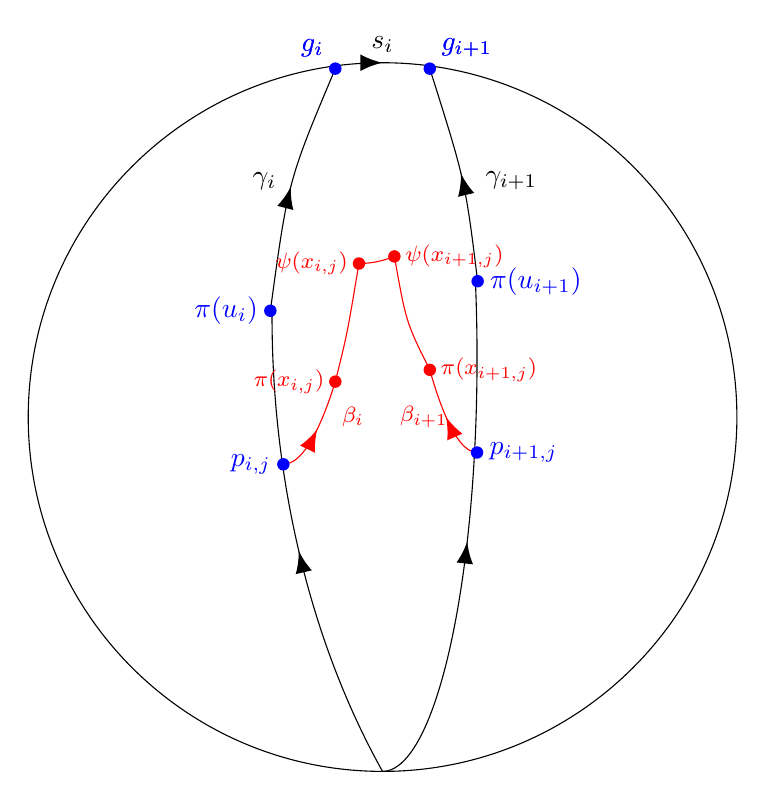
\begin{tikzpicture}[scale=1.5]

 \begin{scope}[decoration={markings,mark = at position 0.5 with {\arrow[scale=2]{latex}}}]

 %
   \draw
    (0,3) circle (3 and 3);



  %u_i
  \draw[postaction={decorate}]
    (0,0) arc (320:360:-4 and 6.0);
  \draw[postaction={decorate}]
    (0,0) arc (-90: 10:0.8 and 3.5);
        % \draw  (-1,2) node {$u_i$};
        %     \draw  (1,2) node[right=-9pt]  {$u_{i+1}$};




       \draw[postaction={decorate}]  (0,6) node[above] {$s_i$};


    %paths gamma_i
    \draw[postaction={decorate}]%[decorate, decoration=snake]
      (-.95,3.9)  .. controls (-.8,5)  .. (-.4,5.95) ;
    \draw  (-1,5) node {$\gamma_i$};
          \draw[postaction={decorate}]%[decorate, decoration=snake]
        (.805,4.15)  .. controls (.7,5) .. (.4,5.95);
    \draw  (1,5) node[right=-9pt] {$\gamma_{i+1}$};







  




       \fill[radius=1.5pt,red]
    (-.4,3.3) circle node[ left=.5pt] {\footnotesize$\pi(x_{i,j})$};
       \fill[radius=1.5pt,red]
    (.4,3.4) circle node[ right=.5pt] {\footnotesize$\pi(x_{i+1,j})$};


       \fill[radius=1.5pt,red]
    (-.2,4.3) circle node[ left=.5pt] {\footnotesize$\psi(x_{i,j})$};
       \fill[radius=1.5pt,red]
    (.1,4.36) circle node[ right=.5pt] {\footnotesize$\psi(x_{i+1,j})$};

        \draw[red]
   (-.4,3.3) .. controls (-.3,3.7)  ..  (-.2,4.3) ;
          \draw[red]
         (.4,3.4) .. controls (.2,3.8) ..     (.1,4.36);

             \draw[red]  (-.25,3) node {\footnotesize$\beta_i$};
     \draw[red]  (.35,3) node {\footnotesize$\beta_{i+1}$};

                \draw[red] (-.2,4.3) parabola (.1,4.36);

             \draw[red,postaction={decorate}]     (-.84,2.6) parabola   (-.4,3.3);
                  \draw[red,postaction={decorate}]   (.8,2.7) parabola       (.4,3.4);
                  
                  
                  
                  
                  
                         \fill[radius=1.5pt,blue]
    (-.84,2.6) circle node[ left=1pt] {$p_{i,j}$};
       \fill[radius=1.5pt,blue]
    (.8,2.7) circle node[right=1pt] {$p_{i+1,j}$};


   \fill[radius=1.5pt,blue]
    (-.95,3.9) circle node[left=1pt] {$\pi(u_i)$};
       \fill[radius=1.5pt,blue]
    (.805,4.15) circle node[right=1pt] {$\pi(u_{i+1})$};


   \fill[radius=1.5pt,blue]
    (-.4,5.95) circle node[above left=1pt] {$g_i$};
       \fill[radius=1.5pt,blue]
    (.4,5.95) circle node[above right=1pt] {$g_{i+1}$};



   \fill[radius=1.0pt,blue]
    (-.4,5.95) circle node[above left=1pt] {$g_i$};
       \fill[radius=1.0pt,blue]
    (.4,5.95) circle node[above right=1pt] {$g_{i+1}$};



     \end{scope}
\end{tikzpicture}
\caption{Depiction of a path in $\Gamma(G,S)$ between $p_{i,j} = \pi(a_{i,1}a_{i,2}\dots a_{i,j})$ and $p_{i+1,j} = \pi(a_{i+1,1}a_{i+1,2}\dots a_{i+1,j})$, where $u_i=a_{i,1}a_{i,2}\dots a_{i,|u_i|_S}$ is such that $\psi(u_i) = g_i$.}\label{fig:filling2}
\end{figure}


Thus there is a path in $\Gamma(G,S)$ from $p_{ij}$ to $p_{i+1,j}$ of length at most $2m+2h_{S,\psi}(mn/2+e+m)+1$
consisting of the following segments, as shown in Figure~\ref{fig:filling2}:
\begin{itemize}[itemsep=5pt]
\item $\beta_i=\{b_{i,j,r}\}_{i=1}^r$ from $p_{i,j}$ to $\pi(x_i)$ of length at most $m$,
\item a path from $\pi(x_i)$ to $\psi(x_i)$ of length at most $h_{S,\psi}(mn/2+e+m)$,
\item an edge labeled $s_i$ from $\psi(x_{i,j})$ to $\psi(x_{i+1,j})$,
\item a path from $\psi(x_i)s_i = \psi(x_{i+1})$ to $\pi(x_{i+1})$ of length at most $h_{S,\psi}(mn/2+e+m)$,
\item $\beta_{i+1}=\{b_{i+1,j,r}\}_{i=1}^r$ from $\pi(x_i)$ to $p_{i+1,j}$ of length at most $m$.
\end{itemize}

In Figure~\ref{fig:filling3} the paths between $p_{i,j}$ and $p_{i+i,j}$ for all $1 \leq j < \max\{|u_i|_S,|u_{i+1}|_S\}$ are  depicted for one corridor.
Between $p_{|u_i|}$ and $p_{|u_{i+1}|}$ we use that existing path
$\gamma_i s_i \gamma_{i+1}^{-1}$.

These corridors create two types of cells.  The first
type are created from two of these paths and their connecting edges, for some $j$ and $j+1 < \max\{|u_i|_S,|u_{i+1}|_S\}$.
This creates a cell with perimeter at most
\[2(2m+2h_{S,\psi}(mn/2+e+m)+1) + 2 = 4m+4h_{S,\psi}(mn/2+e+m)+4,\] where the additional $+2$ accounts for the single edges $a_{i,j+1}$   between $p_{i,j}$ and $p_{i,j+1}$, and   $a_{i+1,j+1}$  between $p_{i+1,j}$ and $p_{+1,j+1}$, which lie on the paths $u_i$ and $u_{i+1}$, respectively, and are not part of the paths previously constructed.



\begin{figure}[h!]
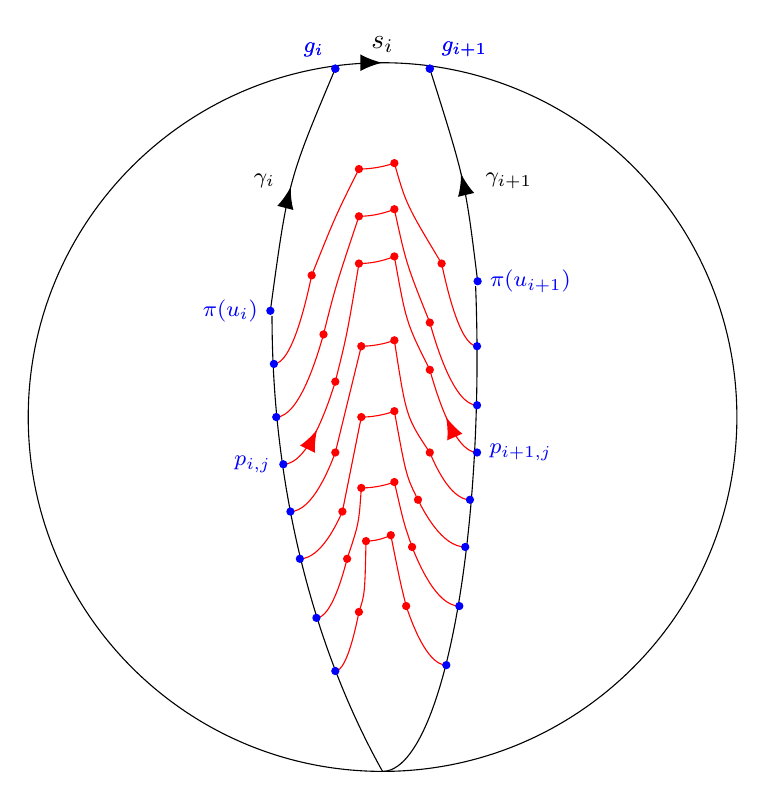
\begin{tikzpicture}[scale=1.5]

 \begin{scope}[decoration={markings,mark = at position 0.5 with {\arrow[scale=2]{latex}}}]

 %
   \draw
    (0,3) circle (3 and 3); %%too perfect, replace


  %u_i
  \draw%[postaction={decorate}]
    (0,0) arc (320:360:-4 and 6.0);
  \draw%[postaction={decorate}]
    (0,0) arc (-90: 10:0.8 and 3.5);
%        \draw  (-1,2) node {$u_i$};
%            \draw  (1,2) node[right=-9pt]  {$u_{i+1}$};




       \draw[postaction={decorate}] (0,6) node[above] {$s_i$};

    %paths gamma_i
    \draw[postaction={decorate}]%[decorate, decoration=snake]
      (-.95,3.9)  .. controls (-.8,5)  .. (-.4,5.95) ;
    \draw  (-1,5) node {\footnotesize$\gamma_i$};
          \draw[postaction={decorate}]%[decorate, decoration=snake]
        (.805,4.15)  .. controls (.7,5) .. (.4,5.95);
    \draw  (1,5) node[right=-9pt] {\footnotesize$\gamma_{i+1}$};







       \fill[radius=1.0pt,red]
    (-.4,3.3) circle ;
       \fill[radius=1.0pt,red]
    (.4,3.4) circle ;

%       \fill[radius=1.0pt,red]
%    (-.2,4.3) circle node[ left=.5pt] {\footnotesize$x_i$};
%       \fill[radius=1.0pt,red]
%    (.1,4.36) circle node[ right=.5pt] {\footnotesize$x_is_i$};
       \fill[radius=1.0pt,red]
    (-.2,4.3) circle; % node[ left=.5pt] {\footnotesize$x_i$};
       \fill[radius=1.0pt,red]
    (.1,4.36) circle ; %node[ right=.5pt] {\footnotesize$x_is_i$};


        \draw[red]
   (-.4,3.3) .. controls (-.3,3.7)  ..  (-.2,4.3) ;
          \draw[red]
         (.4,3.4) .. controls (.2,3.8) ..     (.1,4.36);


                \draw[red] (-.2,4.3) parabola (.1,4.36);
             \draw[red,postaction={decorate}]     (-.84,2.6) parabola   (-.4,3.3);
                  \draw[red,postaction={decorate}]   (.8,2.7) parabola       (.4,3.4);


%                         \draw[red]  (-.25,3) node {\footnotesize$\alpha_i$};
%    \draw[red]  (.35,3) node {\footnotesize$\beta_{i}$};
%
%







    %%%Copy red loops



        \draw[red]
   (-.5,3.7) .. controls (-.4,4.1)  ..  (-.2,4.7) ;
          \draw[red]
         (.4,3.8) .. controls (.2,4.3) ..     (.1,4.76);

                \draw[red] (-.2,4.7) parabola (.1,4.76);
             \draw[red]    (-.9,3) parabola   (-.5,3.7);
                  \draw[red]   (.8,3.1) parabola       (.4,3.8);



    %%%Copy red loops

        \draw[red]
(-.6,4.2) .. controls (-.4,4.7)  ..     (-.2,5.1) ;%C-E
          \draw[red]
         (.5,4.3) .. controls (.2,4.8) ..      (.1,5.15);%D-F

                \draw[red] (-.2,5.1) parabola (.1,5.15); %E-F
             \draw[red]    (-.92,3.45) parabola   (-.6,4.2) ; %A-C
                  \draw[red]   (.8,3.6) parabola     (.5,4.3) ; %B-D



        \draw[red]
    (-.4,2.7) .. controls (-.4,2.7)  ..     (-.18,3.6) ;%C-E
          \draw[red]
           (.4,2.7).. controls (.2,3) ..         (.1,3.65);%D-F

                \draw[red]  (-.18,3.6) parabola     (.1,3.65); %E-F
             \draw[red]      (-.78,2.2)  parabola    (-.4,2.7) ; %A-C
                  \draw[red]      (.74,2.3) parabola      (.4,2.7) ; %B-D





    %%%Copy red loops

        \draw[red]
  (-.34,2.2) .. controls (-.3,2.4)  ..     (-.18,3) ;%C-E
          \draw[red]
         (.3,2.3) .. controls (.2,2.5) ..         (.1,3.05);%D-F

                \draw[red]  (-.18,3) parabola     (.1,3.05); %E-F
             \draw[red]      (-.7,1.8)  parabola    (-.34,2.2); %A-C
                  \draw[red]       (.7,1.9) parabola          (.3,2.3)  ; %B-D





        \draw[red]
    (-.3,1.8)  .. controls (-.2,2.1)  ..        (-.18,2.4) ;%C-E
          \draw[red]
           (.25,1.9)  .. controls (.18,2.1) ..           (.1,2.45);%D-F

                \draw[red]     (-.18,2.4) parabola         (.1,2.45); %E-F
             \draw[red]     (-.56,1.3)  parabola        (-.3,1.8) ; %A-C
                  \draw[red]        (.65,1.4) parabola             (.25,1.9)  ; %B-D



        \draw[red]
 (-.2,1.35) .. controls (-.15,1.5)  ..           (-.14,1.95)  ;%C-E
          \draw[red]
    (.2,1.4)   .. controls (.15,1.6) ..              (.07,2);%D-F

                \draw[red]     (-.14,1.95)  parabola      (.07,2); %E-F
             \draw[red]       (-.4,.85)  parabola       (-.2,1.35); %A-C
                  \draw[red]         (.54,.9) parabola                (.2,1.4)  ; %B-D







           \fill[radius=1.0pt,blue]
    (-.9,3) circle;
       \fill[radius=1.0pt,blue]
    (.8,3.1) circle ;

       \fill[radius=1.0pt,red]
    (-.5,3.7) circle ;
       \fill[radius=1.0pt,red]
    (.4,3.8) circle ;

       \fill[radius=1.0pt,red]
    (-.2,4.7) circle ;
       \fill[radius=1.0pt,red]
    (.1,4.76) circle ;



           \fill[radius=1.0pt,blue]
    (-.92,3.45) circle; %A
       \fill[radius=1.0pt,blue]
    (.8,3.6) circle ; %B

       \fill[radius=1.0pt,red]
    (-.6,4.2) circle ; %C
       \fill[radius=1.0pt,red]
    (.5,4.3) circle ; %D

       \fill[radius=1.0pt,red]
    (-.2,5.1) circle ; %E
       \fill[radius=1.0pt,red]
    (.1,5.15) circle ; %F





           \fill[radius=1.0pt,blue]
    (-.78,2.2) circle; %A
       \fill[radius=1.0pt,blue]
    (.74,2.3) circle ; %B

       \fill[radius=1.0pt,red]
    (-.4,2.7) circle ; %C
       \fill[radius=1.0pt,red]
    (.4,2.7) circle ; %D

       \fill[radius=1.0pt,red]
    (-.18,3.6) circle ; %E
       \fill[radius=1.0pt,red]
    (.1,3.65) circle ; %F


           \fill[radius=1.0pt,blue]
    (-.7,1.8) circle; %A
       \fill[radius=1.0pt,blue]
    (.7,1.9) circle ; %B

       \fill[radius=1.0pt,red]
    (-.34,2.2) circle ; %C
       \fill[radius=1.0pt,red]
    (.3,2.3) circle ; %D

       \fill[radius=1.0pt,red]
    (-.18,3) circle ; %E
       \fill[radius=1.0pt,red]
    (.1,3.05) circle ; %F





           \fill[radius=1.0pt,blue]
    (-.4,.85) circle; %A
       \fill[radius=1.0pt,blue]
    (.54,.9) circle ; %B

       \fill[radius=1.0pt,red]
    (-.2,1.35) circle ; %C
       \fill[radius=1.0pt,red]
    (.2,1.4) circle ; %D

       \fill[radius=1.0pt,red]
    (-.14,1.95) circle ; %E
       \fill[radius=1.0pt,red]
    (.07,2) circle ; %F




           \fill[radius=1.0pt,blue]
    (-.56,1.3) circle; %A
       \fill[radius=1.0pt,blue]
    (.65,1.4) circle ; %B

       \fill[radius=1.0pt,red]
    (-.3,1.8) circle ; %C
       \fill[radius=1.0pt,red]
    (.25,1.9) circle ; %D

       \fill[radius=1.0pt,red]
    (-.18,2.4) circle ; %E
       \fill[radius=1.0pt,red]
    (.1,2.45) circle ; %F



   \fill[radius=1.0pt,blue]
    (-.4,5.95) circle node[above left=1pt] {\footnotesize$g_i$};
       \fill[radius=1.0pt,blue]
    (.4,5.95) circle node[above right=1pt] {\footnotesize$g_{i+1}$};






       \fill[radius=1.0pt,blue]
    (-.84,2.6) circle node[ left=1pt] {\footnotesize$p_{i,j}$};
       \fill[radius=1.0pt,blue]
    (.8,2.7) circle node[right=1pt] {\footnotesize$p_{i+1,j}$};




   \fill[radius=1.0pt,blue]
    (-.95,3.9) circle node[left=1pt] {\footnotesize$\pi(u_i)$};
       \fill[radius=1.0pt,blue]
    (.805,4.15) circle node[right=1pt] {\footnotesize$\pi(u_{i+1})$};


   \fill[radius=1.0pt,blue]
    (-.4,5.95) circle node[above left=1pt] {\footnotesize$g_i$};
       \fill[radius=1.0pt,blue]
    (.4,5.95) circle node[above right=1pt] {\footnotesize$g_{i+1}$};




     \end{scope}
\end{tikzpicture}
\caption{Filling the corridors created by the paths $u_i\gamma_i$ with cells of bounded perimeter.}\label{fig:filling3}
\end{figure}

The second type is the ``top" cell created by the path from $p_{i,|u_i|-1}$ to $p_{i+1,|u_{i+1}|-1}$ together with the path
$a_{i,|u_i|-1}\gamma_is_i\gamma_{i+1}^{-1}a_{i+1,|u_{i+1}|-1}$.
This cell has perimeter at most \[\begin{array}{lll}
&
(2m+2h_{S,\psi}(mn/2+e+m)+1)+2+(  2h_{S,\psi}(mn/2+e)+1)\\
=& 2m+2h_{S,\psi}(mn/2+e+m)+2h_{S,\psi}(mn/2+e)+4\\
\leq & 4m +4h_{S,\psi}(mn/2+e+m)+4\end{array}\]
where the terms in the first line come, respectively, from
\begin{itemize}[itemsep=5pt]
    \item the path from $p_{i,|u_i|-1}$ to $p_{i+1,|u_{i+1}|-1}$,
    \item the two edges labeled $a_{i,|u_i|-1}$ and $a_{i+1,|u_{i+1}-1}$, and
    \item the path $\gamma_is_i\gamma_{i+1}^{-1}$.
\end{itemize}
To obtain the inequality, note that $h_{S,\psi}\in \F$ and $m\geq 1$, so $2m+4\leq 4m+4$ and \[2h_{S,\psi}(mn/2+e+m)+2h_{S,\psi}(mn/2+e)\leq 4h_{S,\psi}(mn/2+e+m).\]
Setting $c=m/2, d=e+m$ and $\cC=4m+4$ proves the first claim in the proposition.

To prove the second claim in the proposition, we count the total number of cells required to subdivide the initial loop into cells of bounded perimeter.
This will yield the inequality involving the Dehn function $\delta$.

It follows from Lemma~\ref{lem:bound1} that $|u_i|\leq mn/2+e$
for all $1\leq i\leq n$.
Each corridor is filled by at most $(mn/2+e)$ cells, each of perimeter at most $4h_{S,\psi}(cn+d)+\cC$, where $c,d$ and $\cC$ depend on $m$ and $e$.
For  a fixed finite  presentation $\langle S\mid R\rangle$ for $G$ with Dehn function $\delta$, each cell constructed above can be filled by at most  $\delta(4h_{S,\psi}(cn+d)+\cC)$ cells with perimeter labeled by a relator from the set $R$.

With $n$ corridors, there are $n\cdot (mn/2+e)=n(cn+e)$ such cells to fill.
Thus an upper bound on the number of relators required to fill $w$ is
\begin{dmath*}
n(cn+e)\cdot \delta\left(4h_{S,\psi}(cn+d)+\cC\right)
=n^2(c+\frac{e}{n})\cdot \delta\left(4h_{S,\psi}(cn+d)+\cC\right)\\
\leq n^2(c+e)\cdot \delta\left(4h_{S,\psi}(cn+d)+\cC\right).
\end{dmath*}
Setting $D=c+e$
and noting that it follows from Lemma~\ref{lemma:lose_the_constant} that $4h_{s,\psi}(cn+d)+\cC\approxF h_{s,\psi}(n)$
proves the second claim of the proposition.
\end{proof}





\section{Separating finitely presented Cayley automatic groups from automatic groups}\label{sec:FP}




In this section we prove Theorem~\ref{thmA:fp}.
First
we  introduce the following  notion.

\begin{definition}
	Let  $f,g\in \F$.
	We say that
	$f \ll g $
	if there exists an unbounded
	function $t \in \F$ such that $ft \preceqF g$. 	
\end{definition}

\begin{example}
If $g(n)=n^c$ with $c>2$ and $f(n)=n^2$ then $f\ll g$.
Take $t(n)=n^{c-2}$.  Then $t \in \F$ is an unbounded function and \[f(n)t(n) = n^c \preceqF g(n).\]
\end{example}

Next we define the following.

\begin{definition}\label{defn:strong-super}
     	A function $f\in \F$ is
{\em  super-quadratic} if for all constants
 	$M > 0$ we have $f(n) \leqslant M n^2$
 	for at most finitely many $n \in \mathbb{N}$.
    A non-zero function is $f\in \F$ is {\em  strongly-super-polynomial} if $n^2f\ll f$.
\end{definition}


\begin{example}
The functions $n^2\ln n$ and  $n^c$ for $c>2$ are super-quadratic;  the functions $e^n$ and  $n^{\ln n}$ are strongly-super-polynomial.
\end{example}

\Olshan\ introduces the notion of a function being {\em almost quadratic} in \cite{Ol-almost}; our definition of a super-quadratic function is the same as being not almost quadratic.
However, our notion of a strongly-super-polynomial is
stronger than the more standard definition of a super-polynomial function given, for example, in \cite{GrigPak}:

\begin{definition}\label{defn:superpoly}
   A function $f:\N\to \R$
   is
   {\em super-polynomial} if $$ \lim_{n \to \infty} \frac{\ln f(n)}{\ln n} = \infty.$$
\end{definition}

In Lemma~\ref{lem:NotStrongSuperP} in the Appendix we give an example of a function in $\F$ which satisfies the above limit but is not strongly-super-polynomial. However  Proposition~\ref{prop:strong_implies_super} justifies our use of ``strongly" since it shows that every strongly-super-polynomial function is super-polynomial.

Proposition~\ref{prop:strongSuper} shows that $f$ is strongly-super-polynomial if and only if $n^cf\ll f$ for any $c>0$, that is, there is nothing special about the choice of the exponent $2$ in Definition~\ref{defn:strong-super}.





\begin{lemma}\label{lem:equiv-super-quad}
	A function $f \in \F$
    is super-quadratic if
    and only if
    $n^2 \ll f$.
\end{lemma}
\begin{proof}
    Assume first that $n^2 \ll f$.
    Since $n^2 \ll f$, there exist an unbounded
    function $t \in \mathcal{F}$ and integer constants
    $K,N>0$ and $M \geqslant 1 $ such that
    $n^2 t(n) \leqslant  K f (M n)$ for all
    $n \geqslant N$.
    Assume that for some $M'\geqslant 1$ there exist
    infinitely many $n_i \in \mathbb{N}$, $i\geq 1$ with $1\leq n_i < n_{i+1}$ for which
    $f(n_i) \leqslant M' n_i^2$.
    Let $n_i = k_i M + r_i$, where $k_i$ is an integer
    and $0 \leqslant r_i < M$. Then we have:
    \begin{equation*}
    \begin{split}
       \frac1{K}  k_i ^2  t(k_i)\leqslant f (M k_i)
        \leqslant f (n_i)
        \leqslant M' n_i^2 = M' M^2 k_i^2 +
        2 M' M r_i k_i + M' r_i ^2 \leqslant \\
        M' M^2 k_i ^2 + 2 M' M^2 k_i + M' M^2
        \leqslant M' M^2 (k_i +1)^2
    \end{split}
    \end{equation*}
    for all $k_i \geqslant N$.
    Therefore, $t(k_i) \leqslant KM'M^2
    \frac{(k_i + 1)^2}{k_i^2} \leqslant 2 KM'M^2$ for all
    $k_i \geqslant \max\{N, 3\}$, where the $3$ follows from
    the simple observation that if
    $k \geqslant 3$ then $\frac{(k+1)^2}{k^2} \leqslant 2$.
    This contradicts the fact that $t$ is an unbounded function.

    Now assume that $f$ is super-quadratic. Then
    for each integer $i \geqslant 1$ the set
    \[ \{m \, |\,\forall n
    \left[n \geqslant m \implies f(n) \geqslant i n^2
    \right]\}\] is non-empty. Let $m_i=\min  \{m \, |\,\forall n
    \left[n \geqslant m \implies f(n) \geqslant i n^2
    \right]\}$.
    We define a function $t(n)$ as follows:
     for $0 \leqslant n < m_1$, let $t(n)=0$, and for
 $m_i \leq n < m_{i+1}$ with $i\geq 1$,  let $t(n) = i$.
    By construction, $t(n)$ is a nondecreasing and unbounded function.
    As $n^2 t(n) \leqslant f(n)$, it follows
    that $n^2 \ll f$.
 \end{proof}





 In \cite{WeirdQuadDehn}  \Olshan\ gives an example of a finitely presented group  which has Dehn function bounded above  by $c_1n^2$ for infinitely many values of $n$,  bounded below by $c_2n^2\log' n\ \log'\log' n$ for infinitely many values of $n$, where $\log'(n)=\max\{\log_2 n, 1\}$, and bounded between $c_3n^2$ and $c_4n^2\log'n\ \log'\log' n$ for all $n\in \N$. Since this Dehn function is not super-quadratic, it follows that  Theorem~\ref{thmA:fp} below does not apply to this example.


We are now ready to prove Theorem~\ref{thmA:fp}.

\ThmA*
\begin{proof}
Fix a presentation for $G$ and let $\delta$ be the Dehn function arising from this presentation. Fix a Cayley automatic structure $(S,S,L,\psi)$ for $G$.
If  $n^2 \ll \delta$,  there is an unbounded function $t(n) \in   \F$ and positive constants $K,M,N_0 \in \N$ so that $n^2t(n) \leq K\delta(Mn)$ for all $n \geq N_0$.



From Proposition~\ref{prop:dehnbound} we know that there are constants $N_1, D\geq 1$ and a function $f\in \F$ so that  for $n \geq N_1$, we have  $\delta(n) \leq Dn^2\delta(f(n))$ where $f\approxF h_{S,\psi}(n)$.

Combining these equations we have  that for all $n\geq \max\{N_0,N_1\}$
\[n^2t(n)\leq K\delta(Mn)\leq KDn^2\delta\left(f(Mn)\right)\]
and dividing both sides by $KDn^2$ we obtain
\begin{equation}\label{egnINEQ}
\frac{t(n)}{KD}\leq  \delta\left(f(Mn)\right).\end{equation}


Define
$$\phi(n) = \min\left\{m\, \middle|\,\frac{t(n)}{KD} \leq \delta(m)\right\}.$$

It is immediate from Equation~(\ref{egnINEQ}) that in the definition of $\phi(n)$ we have $\phi(n) \leq f(Mn)$ for all $n\geq \max\{N_0,N_1\}$, and hence $\phi \preceqF f$.  Since $t \in   \F$ is unbounded, it follows that $\phi \in \F$ and $\phi$ is unbounded.


Now assume that the inequality $n^2 \delta \ll \delta$
is satisfied.
Therefore, there exist integer constants $K,M,N_0 >0$ and an unbounded function $t \in \mathcal{F}$ such that
    \begin{equation}
    \label{ineq_n^2_delta_ll_delta}
      n^2 \delta (n) t(n) \leqslant K \delta (M n)
    \end{equation}
    for all $n \geqslant N_0$.
    It follows from statement (2) of Proposition 3.2. that there exists
    a function $f \approx_1 h_{S,\psi}$ and integer constants
    $N_1 \geqslant 0$ and $D>0$ for which
    the inequality
    \begin{equation*}
     \delta(n) \leqslant D n^2 \delta (f(n))
    \end{equation*}
    holds for all $n \geqslant N_1$.
    This implies that
    $\delta (Mn) \leqslant DM^2 n^2 \delta (f (Mn))$ for all
    $n \geqslant N_1$.
    Combining this with the inequality in \eqref{ineq_n^2_delta_ll_delta} we obtain
    that
    $$n^2 \delta (n) t(n) \leqslant K \delta (M n)
     \leqslant D K M^2 n^2 \delta (f(Mn))
    $$
    for all $n \geqslant  \max \{N_0, N_1\}$.
    Therefore,
    \begin{equation*}
       \delta (n) \tau (n) \leqslant  \delta (f(Mn))
    \end{equation*}
    for all $n \geqslant  \max \{N_0, N_1\}$, where
    $\tau (n) =  \frac{t(n)}{D K M^2}$.
    Let \[m_0 = \min\{n\in \dom(\tau)\subseteq  \N \, | \, \tau(n) \geqslant 2 \};\]
    such $m_0$ exists because $\tau(n)$ is unbounded.
    Therefore,
    \begin{equation*}
    \label{semifinal_ineq}
       2 \delta (n) \leqslant \delta (f(Mn)))
    \end{equation*}
    for all $n \geqslant \max \{N_0, N_1, m_0\}$.
    Let  $d_0 = \min\{n \, | \, \delta (n)
    	\geqslant 1\}$.
    	
    	If $f(Mn)<n$ for some
    $n \geqslant \max\{N_0, N_1, m_0, d_0\}$
    then $2\delta(n)\leq \delta(f(Mn))\leq \delta(n)$, which is a contradiction.
    Thus
for all $n\geq \max \{N_0, N_1, m_0, d_0\}$ we must have that
    \begin{equation*}
    \label{final_ineqAA}
        n \leqslant f(Mn).
    \end{equation*}
   From this we obtain that
   $\ii \preceqF f$. As $f \preceqF h_{S,\psi}$ it follows that
   $\ii\preceqF h_{S,\psi}$, and we conclude that $G$ is $\ii$-separated.
\end{proof}







\section{Dense groups}\label{sec:dense}

We introduce a property of some infinitely presented groups which will allow us to obtain sharper lower bounds on the Cayley distance function of such a Cayley automatic group.
This property will be shown to be independent of generating set and the prototypical examples of groups with this property are wreath products.

Recall that  $F_X$ denotes the free group generated by a set $X$.

\begin{definition}[Densely generated]
\label{def:dense}
Let $G$ be a group with finite  generating set  $X$.
We say that $G$ is   {\em densely generated} by $X$
if  there exist  constants $E,F, N_0\in \N$,
 $1\leq E<F$
such that  for all $n\geq N_0$ there is a word $w_n\in (X\cup X^{-1})^*$ which has the following properties:
 \begin{itemize}[itemsep=5pt]
 \item $w_n=_G1_G$,
 \item $En\leq |w_n|\leq Fn$, and
 \item for any collection of words $u_i,\rho_i\in (X\cup X^{-1})^*$,   $1 \leq j \leq k$ with $u_i=_G1_G$ and
 \[ w_n=_{F_X}\prod_{i=1}^k\rho_iu_i\rho_i^{-1}, \]
 we have $|u_j|>n$ for some  $1 \leq j \leq k$.
 \end{itemize} \end{definition}
In other words, for every interval $[En,Fn]$ there is a loop $w_n$ whose length lies in that interval which  cannot be {filled} by loops all having length at most $n$.
It follows that if $G$ is densely generated by $X$ then every presentation for $G$ over $X$ is infinite.

The following lemma shows that being densely generated is independent of the choice of finite generating set.


\begin{lemma}\label{lem:denseGsetInvariant} If $G$ is {densely generated} by $X$ and $Y$ is another finite generating set for $G$ then $G$ is {densely generated} by $Y$.\end{lemma}




\begin{proof}
Let $| \cdot |_X$ denote the length of a word in $(X \cup X^{-1})^*$ and $| \cdot |_Y$ denote the length of a word in $(Y \cup Y^{-1})^*$.

For each $x\in X$ choose a nonempty word $v_x\in (Y\cup Y^{-1})^*$ with $x=_Gv_x$. Let $M_1=\max_{x\in X}\{|v_x|_Y\}$, and $\tau: (X\cup X^{-1 })^*\to (Y\cup Y^{-1})^*$ be  the monoid homomorphism defined by $\tau(x)=v_x$.
For each $y\in Y$ choose a nonempty word $q_y\in (X\cup X^{-1})^*$ with $y=_Gq_y$. Let $M_2=\max_{y\in Y}\{|q_y|_X\}$, and $\kappa: (Y\cup Y^{-1 })^*\to (X\cup X^{-1})^*$ the monoid homomorphism defined by $\kappa(y)=q_y$.

As $G$ is densely generated by  $X$, there exist fixed constants $E,F,N_0 \in \N$ as in Definition~\ref{def:dense}.
Suppose $G$ is not densely generated by $Y$. Then for all constants $E',F', N_0' \in \N$ there exist some $s\geq N_0'$
so that all words equal to $1_G$ of length between $E's$ and $F's$ can be filled by cells of perimeter at most $s$.

Choose $E'=EM_2$ and $F'=M_1M_2F$, and $N_0'=\max\{N_0,M_1M_2+1\}$.
Let $s_0$ be chosen so that with respect to these constants, all words equal to $1_G$ of length between $E's_0$ and $F's_0$ can be filled by cells of perimeter at most $s_0$.

As $G$ is densely generated by $X$, choose $n=M_2s_0$. There must be a word $w_n\in (X\cup X^{-1})^*$ so that $w_n =_G 1_G$ and whose length satisfies
\[E(M_2s_0)\leq |w_n|\leq F(M_2s_0)\]
which cannot be filled by cells all of perimeter at most $n$.
Then $\tau(w_n)$ labels a path in $\Gamma(G,Y)$ so that
\[EM_2s_0\leq |\tau(w_n)|\leq M_1FM_2s_0.\]
Note that the map $\tau$ does not decrease length, as $\tau(w_n)$ is obtained by substitution, with no free reduction.

Since $E's_0\leq |\tau(w_n)|\leq F's_0$, by our choice of $s_0$ we can fill this word
by cells of perimeter at most $s_0$. Now consider this van Kampen diagram as a subgraph of $\Gamma(G,Y)$.
Map the entire subgraph, edge-by-edge, into $\Gamma(G,X)$ by applying the map $\kappa$; the boundary of the new subgraph consists of paths of the form $\kappa(\tau(x_i))$, where $w = x_1x_2, \cdots x_n$.
These paths form the boundary of the subgraph in $\Gamma(G,X)$ connecting the original vertices on the path labeled by $w_n$, and have length at most $M_1M_2$.  We have thus created cells of the form $\kappa(\tau(x_i))x_i^{-1}$ of perimeter at most $1+M_1M_2$.
These boundary cells, together with the copy of the van Kampen diagram, provide a filling of $w_n$.

In summary, the filling we have created has cells of two types:
\begin{itemize}
    \item the boundary cells, of perimeter $1+M_1M_2$, and
    \item images of the cells in the van Kampen diagram in $\Gamma(G,Y)$, which had perimeter at most $s_0$; after applying the homomorphism $\kappa$, the image of such a cell has perimeter at most $M_2s_0$.
\end{itemize}




Note that we chose $N_0'=\max\{M_2M_1+1,N_0\}$ so all of these cells have perimeter at most $M_2s_0=n$.
This contradicts the assumption that $G$ is densely generated by $X$.  Thus $G$ is also densely generated by $Y$.
\end{proof}





A group is called {\em dense} if it is densely generated by some, hence any, finite generating set.
This definition is inspired by  Baumslag's paper \cite{baumslag61} about wreath products $G\wr H$.
We prove in Proposition~\ref{prop:BaumslagDense} that if $H$ is infinite then $G\wr H$ is  dense.


\begin{proposition}\label{prop:BaumslagDense}
  Let $G$ and $H$ be finitely generated groups.	  If $G$ is nontrivial and $H$ is infinite, then
     $G \wr H$ is dense.
\end{proposition}
\begin{proof}
Let $G = \langle X \, |\,  P \rangle$ and
$H = \langle Y \, | \, Q \rangle$ be presentations of
the groups $G$ and $H$, where
$X \subseteq G$ and $Y \subseteq H$ are finite generating sets.
For each $h \in H$ choose a geodesic word $u_h \in (Y \cup Y^{-1})^*$ with $\pi(u_h) =_G h$, and let
$U = \{ u_h | h \in H\}$.
Then the wreath product $G \wr  H$ has presentation
\[G \wr  H = \langle  X \cup Y \, | \,
P \cup Q \cup \{[a_1^u,a_2^v]\,|\,
a_1,a_2 \in X, u,v \in U\} \rangle.\]


Let $B_{H,Y} (n)$ denote the ball
of radius $n$ in the group $H$ with respect to the
generating set $Y$.
For a given positive integer $m$, define the set of relators
\[ R_m =P \cup Q \cup  \{[a_1^u,a_2^v]
\mid u,v \in U,u\not=v,\pi(u),\pi(v) \in B_{H,Y}(m)\}.\]


For any set $S \subseteq H$, define the relation
$T_S = \{ (s_1 h,s_2 h) \mid s_1,s_2
\in S, h \in H\}$.
Now we mimic Baumslag's argument for
proving the non-finite presentability of
wreath products, presented in Lemma~3 of  \cite{baumslag61}, see also  \cite{berstein2015}.
Baumslag constructs a group $\BaumGroup$
generated by $G$ and $H$ with the following properties:
\begin{itemize}[itemsep=5pt]
    \item $G^{h_1}  \cap G^{h_2} =\{1_G\} $ for all $h_1,h_2 \in H$ with $h_1 \not= h_2$, and
    \item $\left[ G^{h_1}, G^{h_2}\right]= \{1_G\}$ if and only if $(h_1,h_2) \in T_S$.

\end{itemize}
Note that instead of requiring all conjugacy classes to commute in $\BaumGroup$, we only require this when the conjugating elements form a pair in the relation $T_S$.


Choosing $S = B_{H,Y}(n)$ for any fixed $n$, it follows that in $\BaumGroup $ we have $[G,G^h]\not=e$ for any $h$ for which
$(e,h) \not\in T_S$.
In particular, this holds for any
$h \in B_{H,Y} (2n+1) \setminus B_{H,Y} (2n)$.
Therefore there is a relation $[a_1,a_2 ^h]$ in
$R_{2n+1} \setminus R_{2n} $ which cannot be obtained
as a product of conjugates of the relations from
$R_n$.

Now observe that every loop $w \in (X \cup X^{-1} \cup Y \cup Y^{-1})^*$
of length $|w| \leqslant n$
in the wreath product $G \wr H$
can be represented as a product of
conjugates of relations from $R_n$.
Therefore, a loop of length $8n + 8$,
given by the relation $[a_1,a_2 ^h]$,
cannot be decomposed into
smaller loops of length less or equal than $n$.
Thus, $G \wr H$ is dense.
\end{proof}





\section{Separating non-finitely presented Cayley automatic groups from automatic groups}


The proof of Theorem~\ref{thmB:nfp} relies heavily on the following proposition.


\begin{proposition}
   \label{prop:nonFP}

Let $G$ be a non-finitely presented group with  finite generating set $S$.  Then there exists a non-decreasing step function $\phi_S \in\F$, depending on $G$ and $S$,  and  an infinite sequence of integers $\{n_i\}$ such that $\phi_S(n_i)=n_i$ and for any Cayley automatic structure $(S,S,L,\psi)$ on $G$,
\begin{enumerate}
    \item
    $\phi_S \preceqF h_{S,\psi}$, and
    \item if $G$ is dense then
    $\mathfrak i\preceqF h_{S,\psi}$.
\end{enumerate}
\end{proposition}




\begin{proof}
Since $G$ is not finitely presented, there exists an infinite sequence of words  $w_i\in S^*$ so that
\begin{itemize}[itemsep=5pt]
    \item $w_i =_G 1_G$,
    \item if $w_i=\prod_{j=1}^k \rho_ju_j\rho_j^{-1}$ for some $k \in \N$ and $u_j, \rho_j \in S^*$  for $1\leq j\leq k$, then $|u_j|\geq |w_i|$ for at least one value of $j$, and
    \item $|w_i| = l_i$, and $l_i < l_{i+1}$.
\end{itemize}
Define $\phi_S \in   \F$ by $\phi_S(n) = l_i$ for $l_i \leq  n <  l_{i+1}$.



Let $c,d,\cC$, and $n_0$ be the constants from  Proposition~\ref{prop:dehnbound}. Then for any $i\in\N$ with $l_i\geq n_0$ we can
decompose $w_i$ into  loops $u_{i,j}$ using the algorithm described in Proposition~\ref{prop:dehnbound}, and illustrated in Figures~\ref{fig:filling1}, \ref{fig:filling2} and \ref{fig:filling3}, so that $|u_{i,j}| \leq 4h_{S,\psi}(cl_i+d) + \cC$.
Our choice of $w_i$ ensures that for some $j$ we have  $\phi_S(l_i) = l_i = |w_i| \leq |u_{i,j}|$.



Suppose $l_i \leq n < l_{i+1}$.
It follows that for this choice of $j$,
\[ \phi_S(n) = l_{i}\leq |u_{i,j}| \leq 4h_{S,\psi}(c l_{i} + d) + \cC \leq 4h_{S,\psi}(cn+d)+\cC. \]
It then follows from Lemma~\ref{lemma:lose_the_constant} that
 $\phi_S(n) \preceqF h_{S,\psi}(n)$.



Now suppose that $G$ is densely generated by $X$, so there exist constants $E,F$ and $N_0$ so that for all $n \geq N_0$ there exists a loop $w_n=_G 1_G$ so that
\bi
\item $En \leq |w_n| \leq Fn$, and
\item $w_n$ cannot be subdivided into loops all of whose lengths are bounded above by $n$.  That is, if we write $w_n = \Pi_{i=1}^k \rho_i u_i \rho_i^{-1}$ where each $u_i =_G 1_G$ then for some $i$ we have $|u_i| \geq n$.
\ei
Again it follows from Proposition~\ref{prop:dehnbound} that there are constants $c,d,\cC$ and $n_0$ so that for $n \geq \max(n_0,N_0)$, each $u_j$ in the above decomposition of $w_n$ we have
$|u_j| \leq 4h_{S,\psi}(cFn+d)+\cC.$
Since $G$ is dense, it follows that for some $j$ we have
$$n \leq |u_j|\leq 4h_{S,\psi}(cFn+d)+\cC.$$
As this is true for every $n \in \N$ with $n \geq \max(n_0,N_0)$,
it follows from Lemma~\ref{lemma:lose_the_constant} that $\ii \preceqF h_{S,\psi}$.
\end{proof}

We now prove Theorem~\ref{thmB:nfp}.


\ThmB*
\begin{proof}[Proof of Theorem~\ref{thmB:nfp}]
Let $S$ be a fixed finite generating set for $G$.
Suppose $(Y,Y, L, \psi)$ is a Cayley automatic structure for $G$ with respect to some arbitrary finite generating set $Y$.

It follows from part (2) of
Proposition~\ref{prop:modifyingCAstructure} that  $(S,S,L', \psi')$ is another Cayley automatic structure with $h_{Y,\psi}\approxF h_{S,\psi'}$.
If $G$ is dense, it follows from part (2) of Proposition~\ref{prop:nonFP} that  $\ii\preceqF h_{S,\psi'}\approxF h_{Y,\psi}$.

It follows from part (1) of Proposition~\ref{prop:nonFP} that the function $\phi_S$ is such that $\phi_S\preceqF h_{S,\psi'}\approxF h_{Y,\psi}$.
As $S$ was arbitrary, we conclude that for any Cayley automatic structure with respect to any finite generating set $Y$, the function $\phi_S$ which depends only on the group; this is the step function required to prove the theorem.
\end{proof}

\section{Wreath products with virtually infinite cyclic groups}


In this section we prove that if $H$ is virtually infinite cyclic then the wreath product of any non-trivial Cayley automatic group $G$ with $H$ is Cayley automatic.
Moreover, for any Cayley automatic structure, we see that $G \wr H$ is $\ii$-separated.
It follows, for example, that  iterated wreath products $\Z \wr \Z \wr \cdots \wr \Z$ are  Cayley automatic and $\ii$-separated.



\ThmC*


\begin{proof}
To show that $G \wr H$ is Cayley automatic, we will construct a  Cayley automatic structure for $G\wr H$ based on a given Cayley automatic structure for $G$.
It follows from Proposition~\ref{prop:BaumslagDense} that $G \wr H$ is dense, and then from Theorem~\ref{thmB:nfp}
that $G\wr H$ is $\ii$-separated.



Since $G$ is Cayley automatic, there exists a finite symmetric generating set $S_0$ for $G$, a regular language  $L_0 \subseteq S_0^{*}$,  bijection $\psi_0\colon L_0\to G$, and a 2-tape automaton $\texttt{M}_s$  for each $s\in S_0$ with accepted language $$L(\texttt{M}_s)=\{(u,v)\in L_0\times L_0\mid \psi_0(v)=_G \psi_0(u)s\}.$$
Without loss of generality assume $\psi_0(\varepsilon)=1_G$.


Let $H$ be a finite extension of its cyclic subgroup $\mathbb{Z} = \langle t \rangle$ of index $m+1$,
and denote by $ \langle t \rangle \h_0,  \langle t \rangle \h_1, \dots, \langle t \rangle \h_m$ the
distinct  right cosets of $\Z$, where $\h_0 =1_H$.
Let $$T = \{t, \h_1,\dots,\h_m, t^{-1}, \h_1^{-1}, \dots, \h_m^{-1}\};$$
then  $S = S_0 \cup T$ is a symmetric generating set for $G\wr H$.
We identify a particular spanning tree $\mathcal S$ of the Cayley graph $\Gamma(H,T)$ which consists of a ``spine" corresponding to $\langle t \rangle$, and at each vertex $t^k$  there are $m$ ``spokes" terminating at the $m$ vertices $t^kx_j$ of $H$, for $k\in \Z$ and  $1\leq j\leq m$, as in Figure~\ref{fig:spinespine}.

\begin{figure}[h!]
  \centering
  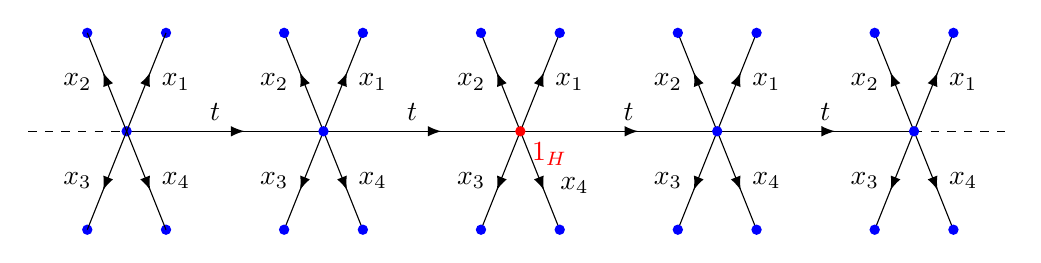
\begin{tikzpicture}[scale=1.25]% rotate=-90]

 \begin{scope}[decoration={markings,mark = at position 0.6 with {\arrow[scale=1.25,black]{latex}}}]


  
       \draw[dashed] (-5,0) -- (-4,0);
      \draw[dashed] (4,0) -- (5,0);
  
       \draw[postaction={decorate}] (-4,0) -- (-2,0);



        \draw[postaction={decorate}] (-2,0) -- (0,0);



  \draw[postaction={decorate}]
         (0,0) -- (2,0);

         
        \draw[postaction={decorate}]
         (2,0) -- ( 4,0);


 
      

\draw (.5,.5) node {$x_1$}; 
\draw (.55,-.55) node {$x_4$}; 
\draw (-.5,.5) node {$x_2$}; 
\draw (-.5,-.5) node {$x_3$}; 
\draw (1.1,.2) node {$t$}; 

\draw (2.5,.5) node {$x_1$}; 
\draw (2.5,-.5) node {$x_4$}; 
\draw (1.5,.5) node {$x_2$}; 
\draw (1.5,-.5) node {$x_3$}; 
\draw (3.1,.2) node {$t$}; 

\draw (4.5,.5) node {$x_1$}; 
\draw (4.5,-.5) node {$x_4$}; 
\draw (3.5,.5) node {$x_2$}; 
\draw (3.5,-.5) node {$x_3$}; 

\draw (-1.1,.2) node {$t$}; 
\draw (-2.5,.5) node {$x_2$}; 
\draw (-2.5,-.5) node {$x_3$}; 
\draw (-1.5,.5) node {$x_1$}; 
\draw (-1.5,-.5) node {$x_4$}; 
\draw (-3.1,.2) node {$t$}; 

\draw (-4.5,.5) node {$x_2$}; 
\draw (-4.5,-.5) node {$x_3$}; 
\draw (-3.5,.5) node {$x_1$}; 
\draw (-3.5,-.5) node {$x_4$}; 

      \draw[postaction={decorate}]
         (0,0) -- ( .4,1);
               \draw[postaction={decorate}]
         (0,0) -- ( .4,-1);
               \draw[postaction={decorate}]
         (0,0) -- ( -.4,1);
               \draw[postaction={decorate}]
         (0,0) -- ( -.4,-1);
         

   \fill[radius=1.5pt,blue]
    (.4,1) circle ;
       \fill[radius=1.5pt,blue]
    (-.4,1) circle ;
       \fill[radius=1.5pt,blue]
    (.4,-1) circle ;
   \fill[radius=1.5pt,blue]
    (-.4,-1) circle ;

         
         
         
               \draw[postaction={decorate}]
         (2,0) -- ( 2.4,1);
               \draw[postaction={decorate}]
         (2,0) -- ( 2.4,-1);
               \draw[postaction={decorate}]
         (2,0) -- ( 1.6,1);
               \draw[postaction={decorate}]
         (2,0) -- ( 1.6,-1);
            \fill[radius=1.5pt,blue]
    (2.4,1) circle ;
       \fill[radius=1.5pt,blue]
    (1.6,1) circle ;
       \fill[radius=1.5pt,blue]
    (2.4,-1) circle ;
   \fill[radius=1.5pt,blue]
    (1.6,-1) circle ;

      \draw[postaction={decorate}]
         (4,0) -- ( 4.4,1);
               \draw[postaction={decorate}]
         (4,0) -- ( 4.4,-1);
               \draw[postaction={decorate}]
         (4,0) -- ( 3.6,1);
               \draw[postaction={decorate}]
         (4,0) -- ( 3.6,-1);
            \fill[radius=1.5pt,blue]
    (4.4,1) circle ;
       \fill[radius=1.5pt,blue]
    (3.6,1) circle ;
       \fill[radius=1.5pt,blue]
    (4.4,-1) circle ;
   \fill[radius=1.5pt,blue]
    (3.6,-1) circle ;




      \draw[postaction={decorate}]
         (-2,0) -- ( -2.4,1);
               \draw[postaction={decorate}]
         (-2,0) -- ( -2.4,-1);
               \draw[postaction={decorate}]
         (-2,0) -- ( -1.6,1);
               \draw[postaction={decorate}]
         (-2,0) -- ( -1.6,-1);
            \fill[radius=1.5pt,blue]
    (-2.4,1) circle ;
       \fill[radius=1.5pt,blue]
    (-1.6,1) circle ;
       \fill[radius=1.5pt,blue]
    (-2.4,-1) circle ;
   \fill[radius=1.5pt,blue]
    (-1.6,-1) circle ;




   \fill[radius=1.5pt,red]
    (0,0) circle node[below right =1pt] {$1_H$};


   \fill[radius=1.5pt,blue]
    (2,0) circle ;


   \fill[radius=1.5pt,blue]
    (4,0) circle ;

   \fill[radius=1.5pt,blue]
    (-2,0) circle ;

   \fill[radius=1.5pt,blue]
    (-4,0) circle ;


            \fill[radius=1.5pt,blue]
    (-4.4,1) circle ;
       \fill[radius=1.5pt,blue]
    (-3.6,1) circle ;
       \fill[radius=1.5pt,blue]
    (-4.4,-1) circle ;
   \fill[radius=1.5pt,blue]
    (-3.6,-1) circle ;
      \draw[postaction={decorate}]
         (-4,0) -- ( -4.4,1);
               \draw[postaction={decorate}]
         (-4,0) -- ( -4.4,-1);
               \draw[postaction={decorate}]
         (-4,0) -- ( -3.6,1);
               \draw[postaction={decorate}]
         (-4,0) -- ( -3.6,-1);




     \end{scope}
\end{tikzpicture}
 \caption{Part of a spanning tree $\mathcal S$ for $\Gamma(H,T)$, where the index of $\Z=\langle t\rangle$ in $H$ is 5.}
 \label{fig:spinespine}
 \end{figure}



We borrow some terminology from the lamplighter groups $\Z_n \wr \Z$ to describe elements of $G \wr H$.
An element $v \in G \wr H$ can be thought of in two equivalent ways:
\begin{itemize}
    \item algebraically, as an element $(\gamma,h)$ where $\gamma \in \bigoplus_{k \in H} (G)_k$ has finitely many nontrivial entries and $h \in H$.
    \item geometrically, as a copy of $\mathcal S$ (or $ \Gamma(H,T)$) where each vertex is marked by some element of $G$, with all but finitely many  vertices marked by $1_G$, and the vertex $h$ of $\mathcal S$ is also marked with a {\em pointer} indicating the final position of the ``lamplighter." We refer to this marking  as a {\em configuration} of ${\mathcal S}$.
\end{itemize}

Write $v = (\gamma,h)$ where
$\gamma \in \bigoplus_{h_i \in H} (G)_{h_i}$ and $h\in H$.
As $H$ is virtually infinite cyclic, we can write $1 \rightarrow K \rightarrow H \rightarrow \Z=\langle t \rangle \rightarrow 1$, where we denote the projection to $\Z$ by $\xi$.
Then the vertex corresponding to $h \in H$ is an endpoint of a spoke attached to the vertex $t^{\xi(h)}$.
For $v = (\gamma,h)$ with $\gamma$ as above, let
\begin{itemize}
    \item $k_* = \xi(h)$,
    \item $k_1 = \min\{0,\xi(h_i) \mid  (g)_{h_i} \in \gamma , (g)_{h_i}\neq 1_G\}$, and
    \item $k_2 = \max\{0,\xi(h_i) \mid  (g)_{h_i} \in \gamma, (g)_{h_i}\neq 1_G \}$.
\end{itemize}
Additionally, let $m_1 = \min(k_*,k_1)$ and $m_2 = \max(k_*,k_2)$.
Define the {\em support} of $v$, denoted $\support(v)$,  to be the interval $[m_1,m_2]$.
The left endpoint of the support is the smallest $k$ so that either
\begin{itemize}
    \item $v$ has a nontrivial entry among the copies of $\Gamma(G,S_0)$ attached to the spine at the vertex $t^k$, including $t^k$ itself,
    \item the final position of the lamplighter is $t^kx_i$ for some $0 \leq i \leq m$, or
    \item all of $k_*$ and $\xi(h_i)$ are positive, that is, the lamplighter is never in a position along the spine with negative index, so $m_1=0$ denotes the starting position of the lamplighter.
\end{itemize}
The right endpoint of the support is defined analogously, where the $0$ is included in the definition of $k_2$ to account for the possibility that $k_*$ and all the $\xi(h_i)$ are negative.




To define our normal form, we
mimic the standard ``left-first" representation of elements of the lamplighter group $\Z_n \wr \Z$ (cf.\   \cite{Taback03}).
Given $v = (\gamma,h) \in G \wr H$, we describe a path traversed by the lamplighter from the vertex $1_H$ in ${\mathcal S}$ to its final vertex $h \in {\mathcal S}$.
If $m_1<0$, the lamplighter first moves left along the spine of ${\mathcal S}$ to the vertex labeled $t^{m_1}$, and marks it with a possibly trivial element of $G$.
The lamplighter then visits $t^{m_1}x_1$ and marks it with a possibly trivial element of $G$ and returns to $t^{m_1}$.
This procedure is repeated for the vertices $t^{m_1}x_2, \cdots ,t^{m_1}x_m$.
The lamplighter then proceeds to the vertex corresponding to $t^{m_1+1}$ and repeats the process of visiting the vertex at the end of each spoke in order and marking it with a possibly trivial element of $G$.
This continues until the lamplighter reaches the vertex corresponding to $t^{m_2}$, where the process is repeated one last time.
If $m_1 \geq 0$, the lamplighter begins the process of marking the vertices with possibly trivial elements of $G$ at $1_H \in {\mathcal S}$, and then visits the spokes as described above, until it reaches the vertex labeled $t^{m_2}$ and marks the vertices $t^{m_2}x_j$ for $0 \leq j \leq m$ with possibly trivial elements of $G$.

We refer to the subpath which starts at the vertex $t^i$ where $i=\min\{m_1,0\}$
as the {\em positive path}, because when written as a word in the group generators, the exponents of $t$ are all positive.
In fact, the positive path is the unique maximal subpath of this word where all exponents of $t$ are positive.




Upon completing the positive path, one of two things will occur.  It may be that the lamplighter is in its final position, and the path simply ends.
If not, the lamplighter moves to its final position via a subpath of the form $t^k$ or  $t^kx_q$ where $k\in \Z, k\leq 0$.
Note that since $m_2$, the right endpoint of $\support(v)$, is the maximum of $k_2$ and $k_*$, the lamplighter will never be in a position along $\Z = \langle t \rangle$ to the right of $m_2$, so the exponent $k$ is non-positive.



Figure~\ref{fig:spine2} shows the configuration of an element with support $[-2,1]$.
\begin{figure}[h!]
  \centering
  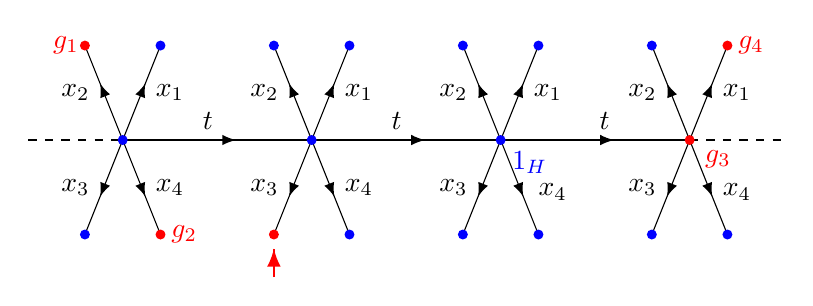
\begin{tikzpicture}[scale=1.2]% rotate=-90]

 \begin{scope}[decoration={markings,mark = at position 1 with {\arrow[scale=1.25,red]{latex}}}]



   \draw[postaction={decorate},red,thick] (-2.4,-1.45) -- (-2.4,-1.15);
   
    \end{scope}

 \begin{scope}[decoration={markings,mark = at position 0.6 with {\arrow[scale=1.25,black]{latex}}}]
  
       \draw[dashed] (-5,0) -- (-4,0);
      \draw[dashed] (2,0) -- (3,0);
  
       \draw[postaction={decorate}] (-4,0) -- (-2,0);



        \draw[postaction={decorate}] (-2,0) -- (0,0);



  \draw[postaction={decorate}]
         (0,0) -- (2,0);

         
        % \draw[postaction={decorate}]
        %  (2,0) -- ( 4,0);


 
      

\draw (.5,.5) node {$x_1$}; 
\draw (.55,-.55) node {$x_4$}; 
\draw (-.5,.5) node {$x_2$}; 
\draw (-.5,-.5) node {$x_3$}; 
\draw (1.1,.2) node {$t$}; 

\draw (2.5,.5) node {$x_1$};  
\draw[red] (2.65,1) node {$g_4$};
\draw[red] (2.3,-.2) node {$g_3$};
\draw (2.5,-.55) node {$x_4$}; 
\draw (1.5,.5) node {$x_2$}; 
\draw (1.5,-.5) node {$x_3$}; 
%\draw (3.1,.2) node {$t$}; 

% \draw (4.5,.5) node {$x_1$}; 
% \draw (4.5,-.5) node {$x_4$}; 
% \draw (3.5,.5) node {$x_2$}; 
% \draw (3.5,-.5) node {$x_3$}; 

\draw (-1.1,.2) node {$t$}; 
\draw (-2.5,.5) node {$x_2$}; 
\draw (-2.5,-.5) node {$x_3$}; 
\draw (-1.5,.5) node {$x_1$}; 
\draw (-1.5,-.5) node {$x_4$}; 
\draw (-3.1,.2) node {$t$}; 

\draw (-4.5,.5) node {$x_2$}; 
\draw[red] (-4.6,1) node {$g_1$}; 
\draw (-4.5,-.5) node {$x_3$}; 
\draw (-3.5,.5) node {$x_1$}; 
\draw (-3.5,-.5) node {$x_4$};  
\draw[red] (-3.35,-1) node {$g_2$}; 


      \draw[postaction={decorate}]
         (0,0) -- ( .4,1);
               \draw[postaction={decorate}]
         (0,0) -- ( .4,-1);
               \draw[postaction={decorate}]
         (0,0) -- ( -.4,1);
               \draw[postaction={decorate}]
         (0,0) -- ( -.4,-1);
   \fill[radius=1.5pt,blue]
    (.4,1) circle ;
       \fill[radius=1.5pt,blue]
    (-.4,1) circle ;
       \fill[radius=1.5pt,blue]
    (.4,-1) circle ;
   \fill[radius=1.5pt,blue]
    (-.4,-1) circle ;

         
         
         
               \draw[postaction={decorate}]
         (2,0) -- ( 2.4,1);
               \draw[postaction={decorate}]
         (2,0) -- ( 2.4,-1);
               \draw[postaction={decorate}]
         (2,0) -- ( 1.6,1);
               \draw[postaction={decorate}]
         (2,0) -- ( 1.6,-1);
            \fill[radius=1.5pt,red]
    (2.4,1) circle ;
       \fill[radius=1.5pt,blue]
    (1.6,1) circle ;
       \fill[radius=1.5pt,blue]
    (2.4,-1) circle ;
   \fill[radius=1.5pt,blue]
    (1.6,-1) circle ;







      \draw[postaction={decorate}]
         (-2,0) -- ( -2.4,1);
               \draw[postaction={decorate}]
         (-2,0) -- ( -2.4,-1);
               \draw[postaction={decorate}]
         (-2,0) -- ( -1.6,1);
               \draw[postaction={decorate}]
         (-2,0) -- ( -1.6,-1);
                     \fill[radius=1.5pt,blue]
    (-2.4,1) circle ;
       \fill[radius=1.5pt,blue]
    (-1.6,1) circle ;
       \fill[radius=1.5pt,red]
    (-2.4,-1) circle ;
   \fill[radius=1.5pt,blue]
    (-1.6,-1) circle ;

      \draw[postaction={decorate}]
         (-4,0) -- ( -4.4,1);
               \draw[postaction={decorate}]
         (-4,0) -- ( -4.4,-1);
               \draw[postaction={decorate}]
         (-4,0) -- ( -3.6,1);
               \draw[postaction={decorate}]
         (-4,0) -- ( -3.6,-1);
            \fill[radius=1.5pt,red]
    (-4.4,1) circle ;
       \fill[radius=1.5pt,blue]
    (-3.6,1) circle ;
       \fill[radius=1.5pt,blue]
    (-4.4,-1) circle ;
   \fill[radius=1.5pt,red]
    (-3.6,-1) circle ;






   \fill[radius=1.5pt,blue]
    (0,0) circle node[below right =1pt] {$1_H$};


   \fill[radius=1.5pt,red]
    (2,0) circle ; 

   \fill[radius=1.5pt,blue]
    (-2,0) circle ;

   \fill[radius=1.5pt,blue]
    (-4,0) circle ;




     \end{scope}
\end{tikzpicture}
 \caption{The element
 $t^{-2}x_2g_1x_2^{-1}x_4g_2x_4^{-1}t^3g_3x_1g_4x_1^{-1}t^{-2}x_3$
 as a configuration of $\mathcal S$. The support of this element is $[-2,1]$ and the arrow denotes the final position of the lamplighter.}
 \label{fig:spine2}
 \end{figure}






As the lamplighter travels along its positive path, we  will wish to  indicate two special positions: the first time the lamplighter is at the vertex corresponding to $1_H=t^0$, and the first time the lamplighter is at the vertex which will be its final position.
The support and the positive path are defined so that these are unique positions along the positive path.

The normal form for the Cayley automatic structure on $G \wr H$ will be constructed in stages.
We first define a normal form $\mathcal N_0\subseteq S^*$  for elements of $G\wr H$ as follows.  Given $v \in G\wr H$ with $\support(v) = [m_1,m_2]$, the above description allows us to uniquely represent $v$ as a word either of the form
\begin{equation}
\label{eqn:nf}
v=t^nx_q\ \text{  or  }\
v=t^{m_1}v_1tv_2\dots tv_st^jx_q
\end{equation}
where $n,j,q, s \in\Z, \ j\leq 0$,
$s\geq 1,  \ 0\leq q\leq m$,  $m_1+(s-1)=m_2$
and
\begin{equation}
\label{eqn:nf2}
v_\cC=v_{\cC,0}\h_1v_{\cC,1}\h_1^{-1}\h_2v_{\cC,2}\dots \h_{m-1}^{-1}\h_mv_{\cC,m}\h_m^{-1}
\end{equation}
where $v_{\cC,t} \in L_0$.  If $m_1 = k_*$ then we allow $v_1$ to be trivial, otherwise $v_1$ must be nontrivial.
If $m_2 = k_*$ we allow $v_s$ to be trivial, otherwise $v_s$ must be nontrivial.
Each word $v_\cC$ encodes a sequence of words $(v_{\cC,0},\dots, v_{\cC,m})\in  L_0^{m+1}$ with $\psi_0(v_{\cC, 0})$ labeling the vertex at position $t^{m_1+\cC-1}$ in $\mathcal S$
and $\psi_0(v_{\cC, i})$ labeling the end of the spoke at position  $t^{m_1+\cC-1}x_i$ for $1 \leq i \leq m$.
Note that in Equation  \eqref{eqn:nf}, the $v_\cC$ are separated by instances of $t$ as the lamplighter moves along the positive path.
Let ${\mathcal N}_0\subseteq S^*$ denote the set of words of this form.


For example,
the element in
 Figure~\ref{fig:spine2}
 has $\mathcal N_0$ normal form
    \begin{equation*}
   \begin{split}
t^{-2}x_1x_1^{-1}x_2v_{1,2}x_2^{-1}x_3x_3^{-1}x_4v_{1,4}x_4^{-1}
 tx_1x_1^{-1}x_2x_2^{-1}x_3x_3^{-1}x_4x_4^{-1}
 tx_1x_1^{-1}x_2x_2^{-1} \\
 x_3x_3^{-1}x_4x_4^{-1}
  tv_{4,0}x_1v_{4,1}x_1^{-1}x_2x_2^{-1}x_3x_3^{-1}x_4x_4^{-1}
 t^{-2}x_3
   \end{split}
   \end{equation*}  where $\psi_0(v_{1,2})=g_1, \psi_0(v_{1,4})=g_2$, $\psi_0(v_{4,0})=g_3$, $\psi_0(v_{4,1})=g_4$, and  in all other cases, $v_{i,j}=\varepsilon$ where $\psi_0(\varepsilon)=1_G$.





We next insert special symbols into the words in $\mathcal N_0$ to obtain the intermediate language $\mathcal N_1$.

Let
$S_1=S\cup\{B,C, B_0,C_*\}$ and
$\Lambda=S_1\setminus T=S_0\cup\{B,C, B_0,C_*\}$.
Let $v = (\gamma,h) \in G \wr H$ be written in the form of Equation~\eqref{eqn:nf}.
Notice that all terms of the form $v_\cC$ are part of the positive path.
With $v_\cC$ as in Equation~\eqref{eqn:nf2}, before each $v_{\cC,j}$ we place the symbol $C$, with one exception.
If $v_{\cC,j}$ is the label of the vertex $h$ of {${\mathcal S}$} which is the final position of the lamplighter, then precede $v_{\cC,j}$ by the symbol $C_*$.
Before each term $v_\cC$ we place the symbol $B$, with one exception.
If $m_1+\cC-1 = 0$ we place the symbol $B_0$ in front of $v_{\cC}$, indicating the unique position along the positive path where the lamplighter is at  the vertex $1_H \in {\mathcal S}$.

Let ${\mathcal N}_1\subseteq S_1^*$ denote the set of all
words in ${\mathcal N_0}$ where the symbols $\{B,C, B_0,C_*\}$ have been inserted as described.
The word  in $\mathcal N_1$ for
the element in
 Figure~\ref{fig:spine2}
is then
\begin{equation*}
  \begin{split}
t^{-2}BCx_1Cx_1^{-1}x_2Cv_{1,2}x_2^{-1}x_3Cx_3^{-1}x_4Cv_{1,4}x_4^{-1}
 tBCx_1Cx_1^{-1}x_2Cx_2^{-1}x_3C_*x_3^{-1} \\
 x_4Cx_4^{-1} tB_0Cx_1Cx_1^{-1}x_2Cx_2^{-1}x_3Cx_3^{-1}x_4Cx_4^{-1}
  tBCv_{4,0}x_1Cv_{4,1}x_1^{-1}x_2Cx_2^{-1} \\ x_3Cx_3^{-1}
  x_4Cx_4^{-1}
 t^{-2}x_3.
   \end{split}
   \end{equation*}






To obtain the final normal form which will be the basis of the Cayley automatic structure for $G \wr H$, let ${\mathcal N}\subseteq \Lambda^*$ denote the set of words in ${\mathcal N}_1$ where all instances of the letters in $T$ are removed.
The word in $\mathcal N$ for
the element in
 Figure~\ref{fig:spine2}
is then
    \begin{dmath*}
BCCCv_{1,2}CCv_{1,4}BCCCC_*C
 B_0CCCCC
  BCv_{4,0}Cv_{4,1}CCC.
   \end{dmath*}



Define the language
\begin{dmath*}
L_1=
 \left\{\prod_{i=1}^p\left(\beta_i\Gamma_{i,0}v_{i,0}\Gamma_{i,1}v_{i,1}\Gamma_{i,2}v_{i,2}\dots \Gamma_{i,m}v_{i,m}\right)\ \middle|\ \begin{array}{ll}
 v_{i,j}~\in L_0,\\
\beta_i~\in\{B,B_0\}, \\ \Gamma_{i,j}~\in \{C,C_\ast \}\end{array}\right\}.
\end{dmath*}
Recall that when $v \neq t^kx_q$,
if $m_1 = k_*$ we allow $v_1$ to be trivial, otherwise $v_1$ must be nontrivial,
and if $m_2 = k_*$ we allow $v_s$ to be trivial, otherwise $v_s$ must be nontrivial.
These conditions are easily verified by a finite state automaton  inspecting, respectively, of the first and last expressions in the product representing an element of $L_1$.
\begin{enumerate}
    \item If $C_*$ occurs in the first factor in the product, then all $v_{i,j}$ may be $\varepsilon$ for $0 \leq j \leq m$; if not, at least one $v_{i,j}$ must be nonempty.
    \item If the $C_*$ occurs in the last factor in the product, then all $v_{i,j}$ may be $\varepsilon$ for $0 \leq j \leq m$; if not, at least one $v_{i,j}$ must be nonempty.
\end{enumerate}
Note that a  finite state automaton can also easily  verify that when all $v_\cC$ are trivial, we have a normal form corresponding to $t^kx_q$.  We assume that all three of these conditions are verified in $L_1$.
As  $L_0$ is a regular language, it follows that $L_1$ is a regular language.

Finally, let
\[ L=L_1\cap \{pB_0qC_\ast r, pC_\ast qB_0r\mid p,q,r\in (\Lambda\setminus\{B_0,C_*\})^*\} . \]
It follows that $L$ is regular and that $L = {\mathcal N}$.


As a further example,
note that if $v = t^nx_q$,
the corresponding word in $L$ is  as follows:
\begin{itemize}[itemsep=5pt]
\item when $n> 0$, we have $\support(t^nx_q) = [0,n]$
and the corresponding  word is \[B_0C^{m+1}(BC^{m+1})^{n-1}B C^qC_*C^{m-q};\]

\item when $n=0$ the corresponding word is $B_0 C^qC_*C^{m-q}$;

\smallskip

\item when $n < 0$, we have $\support(t^nx_q) = [n,0]$ and the corresponding  word is \[B
C^qC_*C^{m-q}
(BC^{m+1})^{n-1}B_0C^{m+1}.\]
\end{itemize}





Given a word $\sigma \in L$, the symbols $B_0$ and $C_*$ allow us to reconstruct the support of the corresponding element, as well as the final position of the lamplighter, that is, the coordinate $h$.
The words $v_{i,j}$ correspond (via $\psi_0$) to elements of $G$ listed in a specified order.  That is, we can deterministically reconstruct $\gamma \in \bigoplus_{h \in H} (G)_h$ and $h \in H$ from $\sigma$.
Formally, let $\tau\colon L \rightarrow \Lambda^*$ be the bijective map defined by
\begin{equation*}
\tau(w) = \tau\left(\prod_{k=1}^s\left(\beta_k\Gamma_{k,0}u_{k,0}\Gamma_{k,1}u_{k,1}\Gamma_{k,2}u_{k,2}\dots \Gamma_{k,m}u_{k,m}\right)\right)  = t^{m_1}v_1tv_2\dots tv_st^j
\end{equation*}
where
\[v_i=v_{i,0}\h_1v_{i,1}\h_1^{-1}\h_2v_{i,2}\dots \h_{m-1}^{-1}\h_mv_{i,m}\h_m^{-1}, \]

\medskip
\noindent
with $u_{i,j} = v_{i,j}$, $\beta_k \in \{B,B_0\}$, $\Gamma_{k,j} \in \{C,C_*\}$ and $m_1$ calculated from the positions of $B_0$ and $C_*$ as described above.


Define $\psi\colon L\to G$ by
 $\psi(w)=\pi(\tau(w))$; by construction, $\psi$  is a bijection.



We claim that $(S,\Lambda,L,\psi)$ is a Cayley automatic structure for $G \wr H$.
To prove this,
we must show that for every generator $s \in S=S_0\cup T$ the set $L_s = \{(u,v) \in L \times L | \psi(u)s =_{G \wr H} \psi(v) \}$ is a regular language, that is, recognized by a 2-tape synchronous automaton.
It suffices to do this for $s \in S_0 \cup \{x_1, \cdots ,x_m,t\}$; see, for example, \cite[Lemma 9]{cga}.


First let $s \in S_0$ and 
suppose $(u,v) \in L_s$.
Viewing $\psi(u)$ as a {configuration} of ${\mathcal S}$ with finitely many vertices marked with elements of $G$
and a distinguished position for the lamplighter,
we can easily see the effect of multiplication  by $s$ on the normal form.
Let $t^kx_q$ denote the vertex of ${\mathcal S}$ which is the final position of the lamplighter in $u$, marked by the element  $g_u \in G$. Let $\rho_u\in L_0$ be such that $\psi_0(\rho_u)=g_u$.
To obtain the normal form word for $\psi(u)s$ we simply multiply $\rho_u$ by $s$ and verify that the multiplication is correct using the multiplier automaton $\texttt{M}_s$ given as part of the given Cayley automatic structure on $G$.
Therefore we need to accept pairs of strings $(u,v) \in L \times L$ of the following form:
\begin{dmath*}
u = \left(\Pi_{i=1}^{p}  \beta_i \Pi_{j=0}^m C \alpha_{i,j}\right)
\Theta_u
\left(\Pi_{i=p+2}^{\cC}  \beta_i   \Pi_{j=0}^m C \alpha_{i,j}\right)
\end{dmath*}
and
\begin{dmath*}
v = \left(\Pi_{i=1}^{p}  \beta_i   \Pi_{j=0}^m C \alpha_{i,j}\right)
\Theta_v
\left(\Pi_{i=p+2}^{\cC}  \beta_i  \Pi_{j=0}^m C \alpha_{i,j}\right)
\end{dmath*}
where $\beta_i \in \{B,B_0\}$, $\alpha_{i,j} \in L_0$,
\[
\Theta_u =  \beta_{p+1}  C\alpha_{p+1,0} \cdots C_* \bm{\alpha_{p+1,r}} \cdots C\alpha_{p+1,m}
\]
and
\[
\Theta_v = \beta_{p+1}  C\alpha_{p+1,0} \cdots C_* \bm{\alpha'_{p+1,r}} \cdots C\alpha_{p+1,m}
\]
where $(\alpha_{p+1,r},\alpha'_{p+1,r})$ is accepted by the multiplier automaton $\texttt{M}_s$ given as part of the given Cayley automatic structure on $G$.  The bold highlighted symbols represent the only difference between the two words.


By
\cite{KKMjournal} (see also \cite[Lemma 8]{cga})  the  language $L_0$ is necessarily quasi-geodesic.
It follows that the difference between the lengths of
$\alpha_{p+1,r}$ and $ \alpha'_{p+1,r}$ is uniformly bounded.
As it is regular to check that two words are identical with a bounded shift, 
it follows that we can construct a 2-tape automaton which checks the prefix of $u$ and $v$ are identical, then calls   $\texttt{M}_s$ to read $(\alpha_{p+1,r},\alpha'_{p+1,r})$, then checks the suffix of $u$ and $v$ are identical.
Thus 
 $L_s$ is a regular language.

Next let $x_i \in \{x_1, \cdots ,x_m\}$, and 
suppose $(u,v) \in L_{x_i}$.
Writing $\psi(u)$ as in Equation~\eqref{eqn:nf}, we see that $\psi(u)x_i$ ends in the letters $x_qx_i$.
The product $x_qx_i \in H$ is an element of some right coset $\langle t \rangle x_r$.  That is, $x_qx_i = t^kx_r$ for some $k$ and $r$.
Viewing $\psi(u)$ and $\psi(v)$ as configurations in ${\mathcal S}$, this means that the configurations are identical except for the final position of the lamplighter which is indicated by $C_*$ in the normal form.
Note that as $x_q$ and $x_i$ vary among the finite set of coset representatives, there are only a finite number of possible values of $(k,r)$ which arise.




The elements $\psi(u)$ and $\psi(v)$ may or may not have identical support. For example 
if  $\psi(u)=t^{-10}g_1t^{20}g_2t^{-5}x_q$ and $x_qx_i=t^{-7}x_r$ then $\support(\psi(u))=\support(\psi(v))$, 
whereas if  $\psi(u)=t^{-10}g_1t^{20}g_2t^{-5}x_q$ and $x_qx_i=t^{-17}x_r$ then $\support(\psi(u))\neq\support(\psi(v))$.


If $\support(\psi(u)) = \support(\psi(v))$,  then we simply need to check the two strings are identical except for the location of $C_*$.  
If $\psi(u)$ ends in $x_q$ when written as in Equation~\eqref{eqn:nf},  we have  $x_qx_i = t^kx_r$.  
Let $\pi:\Lambda^*\to \{C,C_*,B_0\}^*$ be a homomorphism which is the identity on $C,C_*,B_0$ and sends all other letters to $\varepsilon$. 
Then $\pi(u)$ and $\pi(v)$ are identical strings except for the location of $C_*$ in each string. Observe the letter $B_0$ is in the same position in each string since the support of $\psi(u)$ and $\psi(v)$ is the same.
Further observe that there exists an integer  $s_{q,i}$ such that for every pair $(u,v)\in L_{x_i}$ which have the same support, if $C_*$ is the $x$th letter of $\pi(u)$ and the $y$th letter of $\pi(v)$, then $x-y=s_{q,i}$.



 Consider the language $X_{q,i}\subseteq \{C,C_*,B_0\}^*\times  \{C,C_*,B_0\}^*$
consisting of all pairs of strings, each of which contains exactly one $C_*$ letter and one $B_0$ letter, 
where  $C_*$ is the $x$th letter of the first string and the $y$th letter of the second string with $x-y=s_{q,i}$,
and $B_0$ is in the same position in both strings.  
Since these conditions are regular to check, $X_{q,i}$ is a regular language.



Let \[\kappa: \Lambda^*\times \Lambda^*\to  \{C,C_*,B_0\}^*\times  \{C,C_*,B_0\}^*\] be the map which  in each coordinate is the identity on  $C,C_*$ and $B_0$ and sends all other letters  to $\varepsilon$.  
Let $Y \subseteq \Lambda^* \times \Lambda^*$ be the 
language consisting of all pairs of strings 
such that for every positive integer $z$ the $z$th letter of the first
string and the second string is the same unless one of these 
letters is $C_*$ (and the other is $C$). The language $Y$ is regular.    
Then the language \[\kappa^{-1}(X_{q,i})\cap \left(L\times L\right) \cap Y\] is regular, and the union of these languages for $0\leq q\leq m+1$   is exactly the subset of $L_{x_i}$ for which multiplication by $x_i$ does not change the support for the first entry.



Now consider all the possible ways that the support of $\psi(u)$ can change upon multiplication by $x_i$. Again assume $\psi(u)$  ends in $x_q$ when written as in Equation~\eqref{eqn:nf}, and
$x_qx_i = t^kx_r$.  We must consider the following cases.



\begin{enumerate}\item $  \psi(u)=t^nx_q$ and $k\neq 0$,
\item $\psi(u)=t^{m_1}v_1tv_2\dots tv_st^jx_q$ with  $\support(\psi(u))=[m_1,m_2], j\leq 0$ and
\begin{enumerate}\item $k>-j$; in this case  the support  of $v$ extends  further to the right of $m_2$,
\item $k<m_1-m_2-j$; in this case the  support of $v$  extends  further to the left of $m_1$.
\end{enumerate}

\end{enumerate}
Each of these cases can be handled in a manner similar to the above case, by considering the relative positions of $C_*$ and $B_0$ in $\pi(u),\pi(v)$. 
For the first case, if $n>0,k>-n$ then 
 \begin{equation*}
    \begin{split}
    u= B_0C^{m+1}(BC^{m+1})^{n-1}B C^qC_*C^{m-q} \\\text{and } v=B_0C^{m+1}(BC^{m+1})^{n+k-1}B C^rC_*C^{m-r};  \end{split}
    \end{equation*}
if $n>0,k<-n$ then
 \begin{equation*}
    \begin{split}
    u  =  B_0C^{m+1}(BC^{m+1})^{n-1}B C^qC_*C^{m-q}  \\ \text{and } v = B
C^rC_*C^{m-r}
(BC^{m+1})^{-k-n-1}B_0C^{m+1}
    \end{split}
    \end{equation*}
 Analogous pairs of expressions can be worked out for $n\leq 0$; clearly all such pairs can be recognised by 2-tape automata  since $q,i,k,r$ are fixed.
We leave details of the remaining cases to the reader.






Finally, 
suppose $(u,v) \in L_{t}$.
Writing $\psi(u)$ as in Equation~\eqref{eqn:nf}, we see that $\psi(u)t$ ends in the letters $x_qt$. Once again, we can consider the case where the support of $\psi(u)$ does not change, in which case we merely need to check the location of the $C_*$ letters in each word, 
and separately the case where the support of $\psi(u)$ differs at one endpoint from the support of $\psi(v)$.
We follow the same reasoning as in the previous case of multiplication by $x_i$; note that $x_qt$ is in some right coset of $\Z$ in $H$, so we can write $x_qt = t^kx_r$, for a possibly different coset representative $x_r$.
We can  therefore show that  $L_t$ is a regular language as well.
The regular languages $L_s$, $L_{x_i}$ and $L_t$ complete the construction of the Cayley automatic structure
$(S,\Lambda,L,\psi)$ for $G \wr H$, where $H$ is a finite extension of $\Z$.
\end{proof}



\begin{appendix}
\section{Additional results on strongly-super-polynomial functions}


In this appendix we demonstrate the connection between strongly-super-polynomial and super-polynomial functions.

 \begin{proposition}
 \label{prop:strongSuper}	
    Let $0< c < d$. Then for a function $f \in \mathcal{F}$, we have
    $n^{c} f \ll f$ if and only if $n^{d} f \ll f$.
 \end{proposition}
 \begin{proof}
    Assume first that $n^{d} f \ll f$. Then there exists
    an unbounded function $t \in \mathcal{F}$ and integer constants $K,M>0$ and $N \geqslant 0$
    such that
    $n^{c} f(n) t(n) \leq K f (Mn)$ for all
    $n \geq N$.
    Let $\tau  (n)= n^{d-c} t(n)$. Then $\tau \in \mathcal{F}$ and as $t$ is unbounded, so is $\tau$. Writing
    $n^{c} f(n) \tau(n)\leq K f (Mn)$, it follows that
    $n^{c} f \ll f$.

    Now assume that $n^{c} f \ll f$. Then there exists
    an unbounded function $t \in \mathcal{F}$ and
    integer constants $K,M>0$ and $N \geqslant 0$
    such that
    $n^{c} f(n) t(n) \leqslant K f (Mn)$ for all
    $n \geqslant N$. Therefore, the inequality
    \begin{equation*}
        n^{c} t (n) \leqslant K \frac{f(Mn)}{f(n)}.
    \end{equation*}
    holds for all $n \geqslant N$. This implies that
    the inequality
    \begin{equation}
    \label{main_ineq}
       (M^k n)^{c} t(M^k n) \leqslant K \frac{f(M^{k+1}n)}
       {f(M^{k}n)}
    \end{equation}
    holds for all integers $k \geqslant 0$ and $n \geqslant N$.
    Let $k_0 = \lfloor \frac{d}{c}\rfloor$; then we have
    $d \leqslant (k_0+1) c$.
    Allowing $k$ to take all values between $1$ and $k_0$ in \eqref{main_ineq} and multiplying the resulting inequalities together yields
    \begin{dmath*}
    \label{main_ineq2}
        n^{c} t(n) (M n)^{c} t(M n) \dots
       (M^{k_0} n)^{c} t(M^{k_0} n)
       \nonumber \\\leq
       K^{k_0+1} \frac{f(Mn)}{f(n)} \frac{f(M^2 n)}{f(M n)}
       \dots \frac{f(M^{k_0+1}n)}{f(M^{k_0}n)}
       =
       K^{k_0 +1}  \frac{f(M^{k_0 +1}n)}{f(n)}.
    \end{dmath*}





   It follows that
    \begin{equation}
    \label{main_ineq3}
       M' n^{c (k_0+1)}  \tau (n) \leqslant K ^{k_0 +1}
       \frac{f(M^{k_0+1}n)}{f(n)}
    \end{equation}
 holds for all $n \geqslant N$, where
 $\tau (n) = t(n) t(Mn)\dots t(M^{k_0}n)$ and
 $M' =$  $M^{c}$  $M^{2c} \dots M^{k_0 c}$.
 Since $M' \geqslant 1$, the inequality in \eqref{main_ineq3}
 implies that
 \begin{equation}
 \label{final_ineq}
    n^{c (k_0 +1)} f(n) \tau (n) \leqslant
    K^{k_0+1} f(M^{k_0 + 1}n)
 \end{equation}
 for all $n \geqslant N$. By construction, $\tau(n)$ is both an element of ${\mathcal F}$ and an
 an unbounded function.
 Therefore, $n^{c (k_0 + 1)} f \ll f$.
 As $d \leq (k_0+1)c$ it follows from the initial argument in the proof that $n^{d} f \ll f$.
\end{proof}

The following lemma presents an example of  a function which is super-polynomial
but not  strongly-super-polynomial.

\begin{lemma} \label{lem:NotStrongSuperP}
For given $\alpha > 1$, let $f_{\alpha}:\N\to\R $ be the function  defined by $f_{\alpha}(n)= \alpha^{(\ln n)^{1.5} }$. Then \begin{enumerate}
\item $f\in \F$,
\item $f_\alpha$ is super-polynomial, and
\item $f_\alpha$ is not strongly-super-polynomial.  	
\end{enumerate}
\end{lemma}	

\begin{proof}
It is clear that $ f_{\alpha}\in \F$ since $\alpha>1$.

We have \[ \lim_{n \to \infty} \frac{\ln (\alpha^{(\ln n)^{1.5}})}{\ln n}
=\lim_{n \to \infty} \frac{(\ln n)^{1.5}\ln (\alpha)}{\ln n}
=\ln (\alpha)\lim_{n \to \infty} (\ln n)^{0.5}=\infty
\]
so $f_{\alpha}$ is
   super-polynomial. Note that $\alpha>1$ so $\ln \alpha>0$.



   Suppose (for contradiction) that
$f_{\alpha}$ is strongly-super-polynomial, so  there is an unbounded
   function $t \in \mathcal{F}$ and positive integer constants $K,M$ and $N$
   such that $n^2 f_{\alpha}(n) t(n) \leq K f_{\alpha}(Mn)$
   for all $n \geq N$. This means




    \begin{equation*}
    \label{ex_ineq1}
 t(n)  \leq
      \frac{ K\alpha^{(\ln(Mn))^{1.5}-(\ln(n))^{1.5}}}{n^2 }
   \end{equation*}


   Taking the logarithm of this inequality we obtain:
   \begin{dmath*}
    \label{ex_ineq1}
    \ln(t(n))\leq \ln K +\left[(\ln(Mn))^{1.5}-(\ln(n))^{1.5}\right]\ln \alpha-2\ln n
   \end{dmath*}  which we can write
   as
   \begin{dmath*}
    \label{ex_ineq3}
        \ln(t(n))\leq \ln K +\left[(\ln(M)+\ln(n))(\ln(Mn))^{0.5}-(\ln (n))(\ln(n))^{0.5}\right]\ln \alpha-2\ln n
   \end{dmath*}
      which becomes


      \begin{dmath*}
    \label{ex_ineq4}
      \ln( t(n))
      \leqslant \ln K + (\ln( M) )(\ln (Mn))^{0.5}  \ln \alpha +
      (\ln( n) )\left[\left(\ln (Mn))^{0.5}
       - (\ln n)^{0.5} \right) \ln( \alpha)-2 \right]
   \end{dmath*}
         which becomes
      \begin{dmath*}
    \label{ex_ineq4}
      \ln( t(n))
      \leqslant \ln K + (\ln( M) )(\ln (Mn))^{0.5}  \ln \alpha +
     \ln( \alpha) (\ln( n) )\left[\left(\ln (Mn))^{0.5}
       - (\ln n)^{0.5} \right) -\frac{2}{\ln( \alpha)} \right]
   \end{dmath*}




   Now if we let
   $B=\ln (Mn)^{0.5} - (\ln n)^{0.5}$ then
   $B(\ln (Mn)^{0.5} + (\ln n)^{0.5})
   =\ln (Mn)-(\ln n)=\ln M$ and so \[B=\frac{\ln M}{(\ln (Mn))^{0.5}
       + (\ln n)^{0.5}}.\]

   Thus
      \begin{dmath*}
    \label{ex_ineq5}
      \ln( t(n))
      \leqslant \ln K + (\ln( M) )(\ln (Mn))^{0.5} \ln \alpha +
     \ln( \alpha) (\ln( n) )\left[\left(\frac{\ln M}{(\ln (Mn))^{0.5}
       + (\ln n)^{0.5}}\right) -\frac{2}{\ln( \alpha)} \right]
   \end{dmath*}
        which becomes
         \begin{dmath*}
    \label{ex_ineq7}
      \ln( t(n))
      \leqslant \ln K +
     \ln \alpha \ln( M) \left[(\ln (Mn))^{0.5} +
     (\ln( n) )\left[\left(\frac{1}{(\ln (Mn))^{0.5}
       + (\ln n)^{0.5}}\right) -\frac{2}{\ln( \alpha)\ln M} \right]\right]
   \end{dmath*}
   which becomes
   \begin{dmath*}
    \label{ex_ineq8}
      \ln( t(n))
      \leqslant \ln K +
     \ln \alpha \ln( M) \left[\frac{(\ln (Mn))}{(\ln (Mn))^{0.5}} +
     (\ln( n) )\left[\left(\frac{1}{(\ln (Mn)^{0.5}
       + (\ln n)^{0.5}}\right) -\frac{2}{\ln( \alpha)\ln M} \right]\right]
   \end{dmath*}
   which becomes
     \begin{dmath*}
      \ln( t(n))
      \leqslant \ln K +
     \ln \alpha \ln( M) \left[\frac{(\ln (M)+\ln(n))}{(\ln (Mn))^{0.5}} +
     (\ln( n) )\left[\left(\frac{1}{(\ln (Mn)^{0.5}
       + (\ln n)^{0.5}}\right) -\frac{2}{\ln( \alpha)\ln M} \right]\right]
 \end{dmath*}
      which becomes
    \begin{dmath*}
      \ln( t(n))
      \leqslant \ln K +
     \ln \alpha \ln( M) \ln (n)
     \left[ \left[\frac{\ln (M)}{(\ln(n))\ln (Mn))^{0.5}} +
     \frac{1}{(\ln (Mn))^{0.5}} +
    \frac{1}{(\ln (Mn)^{0.5}
       + (\ln n)^{0.5}}\right] -\frac{2}{\ln( \alpha)\ln M} \right]
   \end{dmath*}

   The expression in the inside square brackets is going to  $0$ as $n\to\infty$, so eventually it will be less than $\frac{2}{\ln( \alpha)\ln M}$, contradicting the fact that $t\in\F$.
   \end{proof}







The next proposition proves that any function which is strongly-super-polynomial is also super-polynomial.

       \begin{proposition}
       \label{prop:strong_implies_super}
    Let $f \in \F$ be a non-zero function.
    If $f$ is strongly-super-polynomial, then
    $f$ is super-polynomial.
 \end{proposition}	

 \begin{proof}
    Since $f$ is strongly-super-polynomial, by Proposition~\ref{prop:strongSuper} we have $n^cf\ll f$ for {\em any} arbitrary $c>0$ we wish to choose.
    So for any $c>0$ there are positive constants
    $K_c,M_c$ and $N_c$ and
    an unbounded function $t_c \in \mathcal{F}$
    so that
    the inequality
    \begin{equation*}
    	n^c f(n) t_c(n) \leqslant K_c f(M_cn)
    \end{equation*} 	
    holds for all $n \geq N_c$.
    Therefore, for all $n \geq N_cM_c$ we have
    \begin{equation*}
    \label{str_sup_pol_eq1}
       \left\lfloor \frac{n}{M_c}
       \right\rfloor^c
       f\left( \left\lfloor \frac{n}{M_c}
       \right\rfloor\right)
       t_c\left(\left\lfloor \frac{n}{M_c}
       \right\rfloor\right) \leqslant K_c
       f \left( M_c \left\lfloor \frac{n}{M_c}
       \right\rfloor\right) \leqslant K_c f (n).
    \end{equation*}
    Taking the logarithm of this inequality
    we obtain
    \begin{equation*}
    \label{str_sup_pol_eq2}
       c \ln \left\lfloor \frac{n}{M_c}
       \right\rfloor +
       \ln f\left( \left\lfloor \frac{n}{M_c}
       \right\rfloor\right)  +  \ln t_c \left(\left\lfloor \frac{n}{M_c}
       \right\rfloor\right) \leqslant
       \ln K_c  + \ln f (n).
    \end{equation*}
    which becomes
        \begin{equation*}
    \label{str_sup_pol_eq3}
       c \ln \left\lfloor \frac{n}{M_c}
       \right\rfloor +
       \ln f\left( \left\lfloor \frac{n}{M_c}
       \right\rfloor\right)  +  \ln t_c \left(\left\lfloor \frac{n}{M_c}
       \right\rfloor\right) - \ln K_c\leqslant
         \ln f (n).
    \end{equation*}


    Now since $f$ and $t_c$ are both unbounded functions, there exists some  $N_c'\geq N_cM_c$ so that \[\ln f\left( \left\lfloor \frac{n}{M_c}
       \right\rfloor\right)  +  \ln t_c \left(\left\lfloor \frac{n}{M_c}
       \right\rfloor\right)-\ln K_c\geq 0\]
       for all $n\geq N_c'$. Thus we have
               \begin{equation*}
    \label{str_sup_pol_eq4}
       c \ln \left\lfloor \frac{n}{M_c}
       \right\rfloor
      \leq
         \ln f (n)
    \end{equation*} for all $n\geq N_c'$.

    Dividing sides
    by $\ln n$, we obtain that
         \begin{equation}
    \label{str_sup_pol_eq5}
       c \frac{\ln \left\lfloor \frac{n}{M_c}
       \right\rfloor}{\ln n}
       \leq
         \frac{\ln f (n)}{\ln n}
    \end{equation} for all $n\geq N_c'$.

    Now choose $I_c\in \N$ so that $I_c\geq N_c'$
    and $\frac{\ln \left\lfloor \frac{n}{M_c}
       \right\rfloor}{\ln n}>0.9$ for all $n\geq I_c$. Observe that the limit  $\lim_{n\to\infty}\frac{\ln \left\lfloor \frac{n}{M_c}
       \right\rfloor}{\ln n}=1$ and the term $\frac{\ln \left\lfloor \frac{i}{M_c}
       \right\rfloor}{\ln i}$ is increasing, so such a value $I_c$ exists.

    Then from this observation and equation~(\ref{str_sup_pol_eq5})  we get
      \begin{equation*}
    \label{str_sup_pol_eq6}
     0.9c\leq   c  \frac{\ln \left\lfloor \frac{n}{M_c}
       \right\rfloor}{\ln n}
       \leq
         \frac{\ln f (n)}{\ln n}
    \end{equation*} for all $n\geq I_c$.


    Since $c>0$ can be arbitrary, this shows that the limit of $  \frac{\ln f (n)}{\ln n}$ must go to $\infty$.
    \end{proof}

\end{appendix}
\bibliographystyle{plain}
\bibliography{BET_bibliography}

\end{document}
